The LHC provides a unique opportunity to search for weakly coupled $\mathcal{O}$(GeV) Heavy Neutral Leptons with the ATLAS detector given the large dataset of $W$-bosons. In 2022, the ATLAS experiment performed a search for HNLs, in the same final state targeted in this analysis, with the full Run-2 dataset~\cite{PhysRevLett.131.061803} (referred to as the 2022 analysis throughout this dissertation). However, the ATLAS object reconstruction algorithms have gone through significant improvement~\cite{atlascollaboration2023software} since then, opening up the opportunity to reanalyze the dataset with enhanced techniques and a better overall performance.~\Cref{sec:ana_goals} highlights the improvements in the reconstruction chain that the analysis benefits from and the corresponding new parameter space that these improvements unlock.~\Cref{sec:data_mc_samples} lists out the dataset and the Monte Carlo samples used in this search. Finally,~\cref{sec:object_sel} discusses the requirements imposed on the various objects used in this analysis.


\section{Analysis Goals}\label{sec:ana_goals}

This analysis searches for Heavy Neutral Leptons using 140.1 $fb^{-1}$ of $pp$ collision data recorded at $\sqrt{s}=13$~TeV in the $W\rightarrow \ela \mathcal{N}\left(\rightarrow\elb\elg\nu \right)$ final state. The charged lepton coming from the $W$ decay (\ela) is called the \textit{prompt} lepton since it appears to come from the primary $pp$ collision. Since the HNL is long-lived, the $\elb\elg$ system manifests as a two-pronged Secondary Vertex (SV) or Displaced Vertex (DV)\footnote{secondary, because the $pp$ collision and the $W$ production and decay gives the primary vertex, and displaced, because the the HNL has a proper lifetime long enough to resolve the PV and the SV.}, and \elb~and \elg~are called \textit{displaced} leptons. The ATLAS ID has the highest granularity (in the $\eta-\phi$ directions) out of all the sub-detector systems, making it the most adept at reconstructing the position and the kinematics of this DV. Hence, the analysis uses a reconstructed two-track DV in the ID volume. The reconstruction selection criteria, or cuts, on the ID tracks (specifically the $|d_0|\leq 300$~mm cut and the minimum number of hits) automatically impose a requirement that the DV radial position ($r_\mathrm{DV}$) has to be within the first layer of the strips silicon detectors (see~\cref{fig:inner-det}). Furthermore, the SV is required to be displaced ($r_\mathrm{DV}>4$~mm), adding a minimum requirement on the radial distance between PV and the DV in the radial direction. Finally, \ela, \elb, \elg~are required to be either $\mu$ or $e$, since $\tau$-leptons are unstable and decay rapidly. The electric charge of \ela~follows that of the $W$ boson, while \elb~and \elg~are oppositely charged. The goal of this analysis can hence be summarized as:

\textbf{A search for Heavy Neutral Leptons in decays of $W$ bosons in events with a prompt muon or electron, and a two-track displaced vertex in the Inner Detector volume of ATLAS with outgoing oppositely charged muons or electrons.}

\subsection{Reconstruction improvements}
The final state probed in this analysis in non-standard, since the primary ATLAS reconstruction chain is designed around reconstructing signatures from prompt particle decays, as described in~\cref{sec:reco}. Dedicated reconstruction techniques, such as LRT, add significant sensitivity to this final state. The 2022 analysis used an older, computationally expensive version of LRT which was only run on about 10$\%$ of the events retained by the ATLAS triggers based on a pre-defined set of filters. Furthermore, the LRT pass used for the 2022 analysis reconstructed a significant amount of ``fake" tracks, which inflated the amount of background faced. Lastly, LRT was only run for HNL signal Monte Carlo samples and not for other SM samples, which inhibited the usage of Monte Carlo-driven background estimation techniques. 

The analysis presented in this dissertation overcomes all of these challenges thanks to the vast improvement in reconstruction techniques, specifically in LRT. The new optimized LRT deployed for reconstruction in Run-3~\cite{IDTR-2021-03} was retroactively applied to data collected in Run-2 and all Monte Carlo simulations prepared for Run-2 conditions. The computational costs are significantly lowered, removing the need for filtering of events, making it possible to look for LLP events in all ATLAS data. The optimization significantly reduces the rate of fake tracks (and hence non-LLP SVs) reconstructed by the LRT chain while maintaining high signal efficiency as illustrated in~\cref{fig:LRT-fakeRate}, which compares the number of reconstructed DVs (both, genuine LLP and fake, i.e. non-LLP) between the legacy (implementation used in the 2022 analysis) and updated LRT reconstruction as a function of $r_\mathrm{DV-PV}$ (or $L_\mathrm{xy}$) using as a benchmark a simulated sample of $H\rightarrow aa \rightarrow b\bar{b}b\bar{b}$, where $a$ is an LLP.

\begin{figure}[!ht]
    \centering
    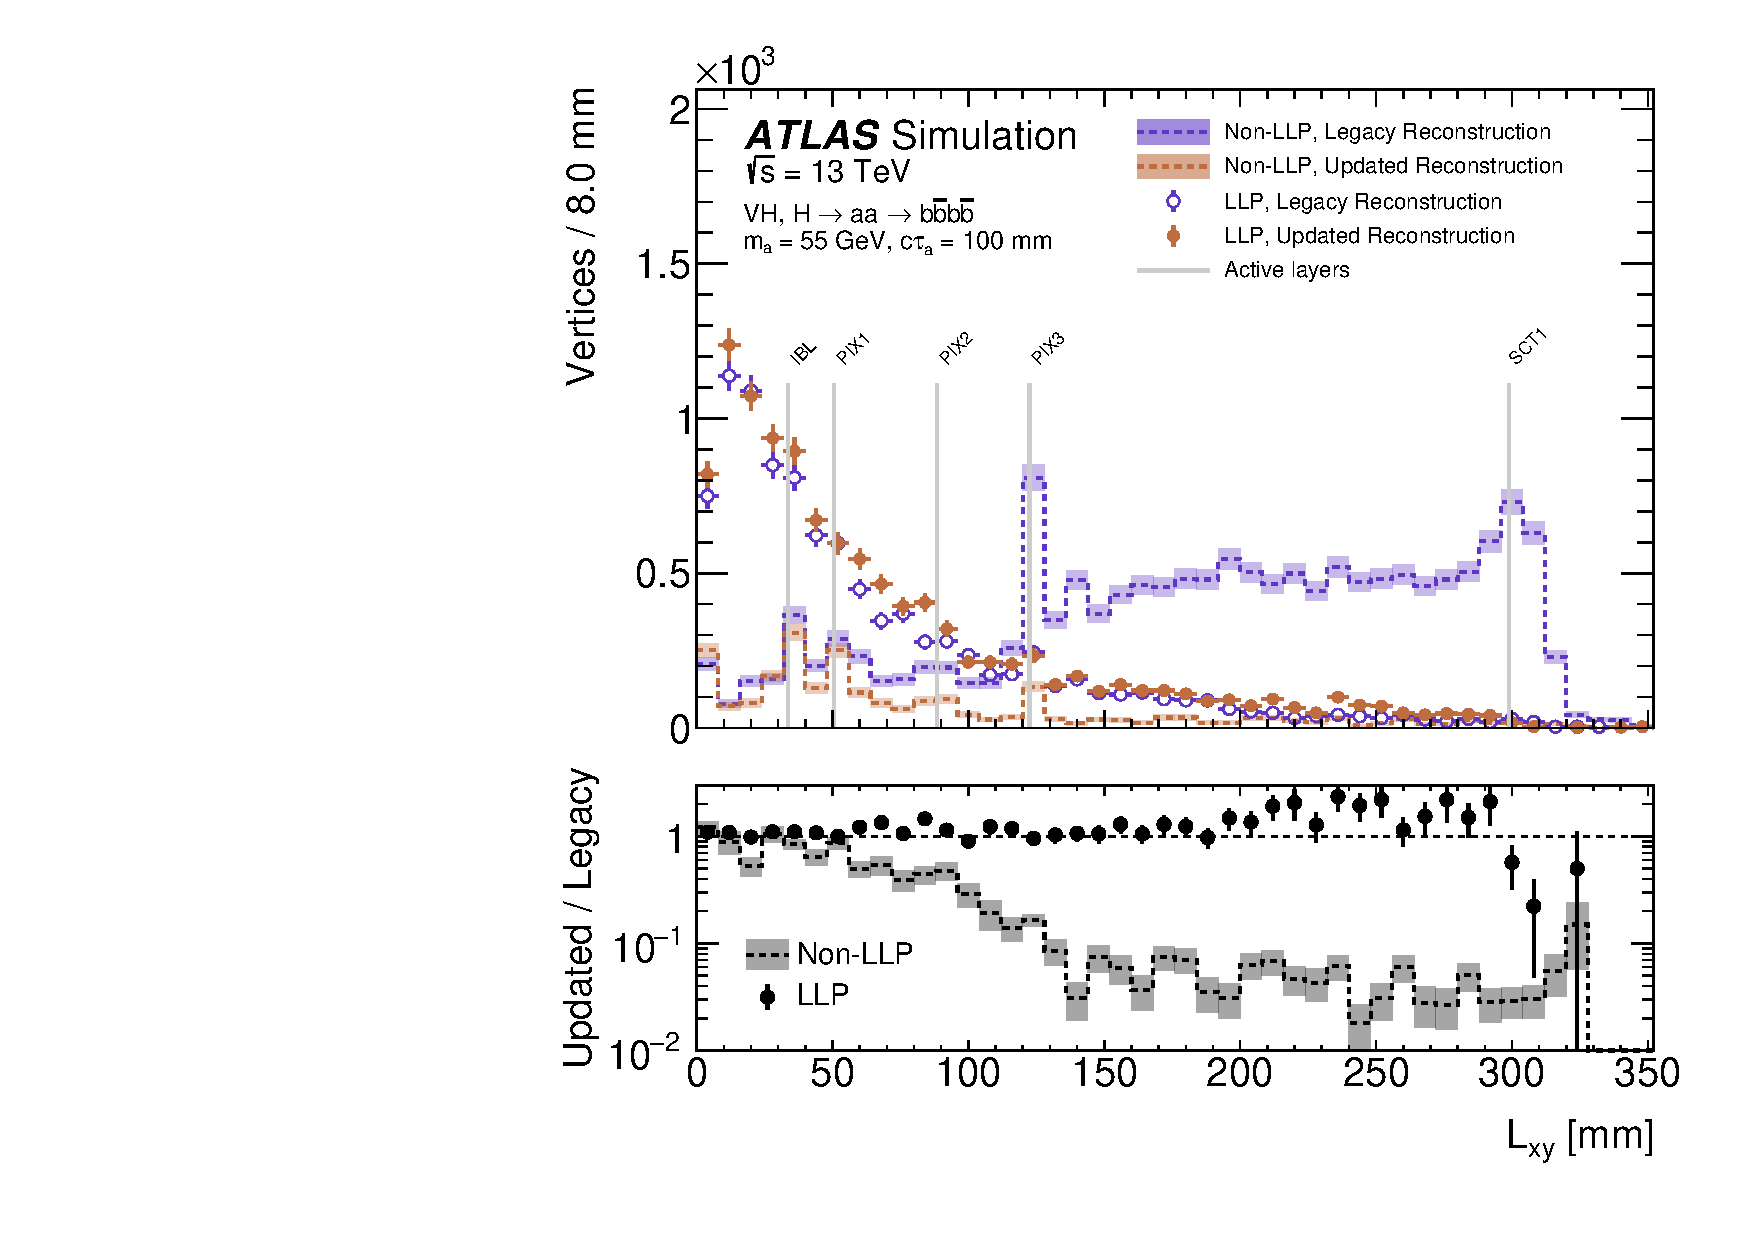
\includegraphics[width=0.6\linewidth]{figures//analysis_overview/LRT_fakeRate.pdf}
    \caption{A comparison of the radial distributions of reconstructed secondary vertices in a simulated LLP sample using the legacy and updated track reconstruction configurations.~\cite{IDTR-2021-03}}
    \label{fig:LRT-fakeRate}
\end{figure}


\subsection{Target Phase Space}

The vast improvements in LRT warrant a new search for displaced HNLs in leptonic final states using the full Run-2 dataset.~\Cref{fig:HNL-summ-mu} summarizes the current limits imposed on the square of the coupling of the HNL to a muon neutrino ($|U_{\mu\mathcal{N}}|^2$) in a single-flavor mixing scenario. The 2022 ATLAS analysis, shown in grey, excluded HNLs in the 1-10 GeV mass range with the corresponding lower limits on $|U_{\mu\mathcal{N}}|^2$ lying in the 10$^{-4}$ and 2$\cdot$10$^{-7}$ order. The analysis described in this thesis aims to expand the 2022 exclusion contour in all directions. Specifically, expansion to lower couplings in the 1-3 GeV \mhnl range probes HNL parameter spaces untouched by any other experiment. Furthermore, expanding to exclude \mhnl$>$10 GeV with couplings smaller than 10$^{-6}$ allows the exploration of completely new parameters. The former goal is achievable by more advanced background estimation methods, since the $\mathcal{O}$(GeV) \mhnl regions are generally dominated by background from hadronic decays. The latter goal is achievable by exploiting the improved LRT and DV reconstruction, since that phase space is limited by background with DVs from uncorrelated track crossings.

\begin{figure}[!ht]
    \centering
    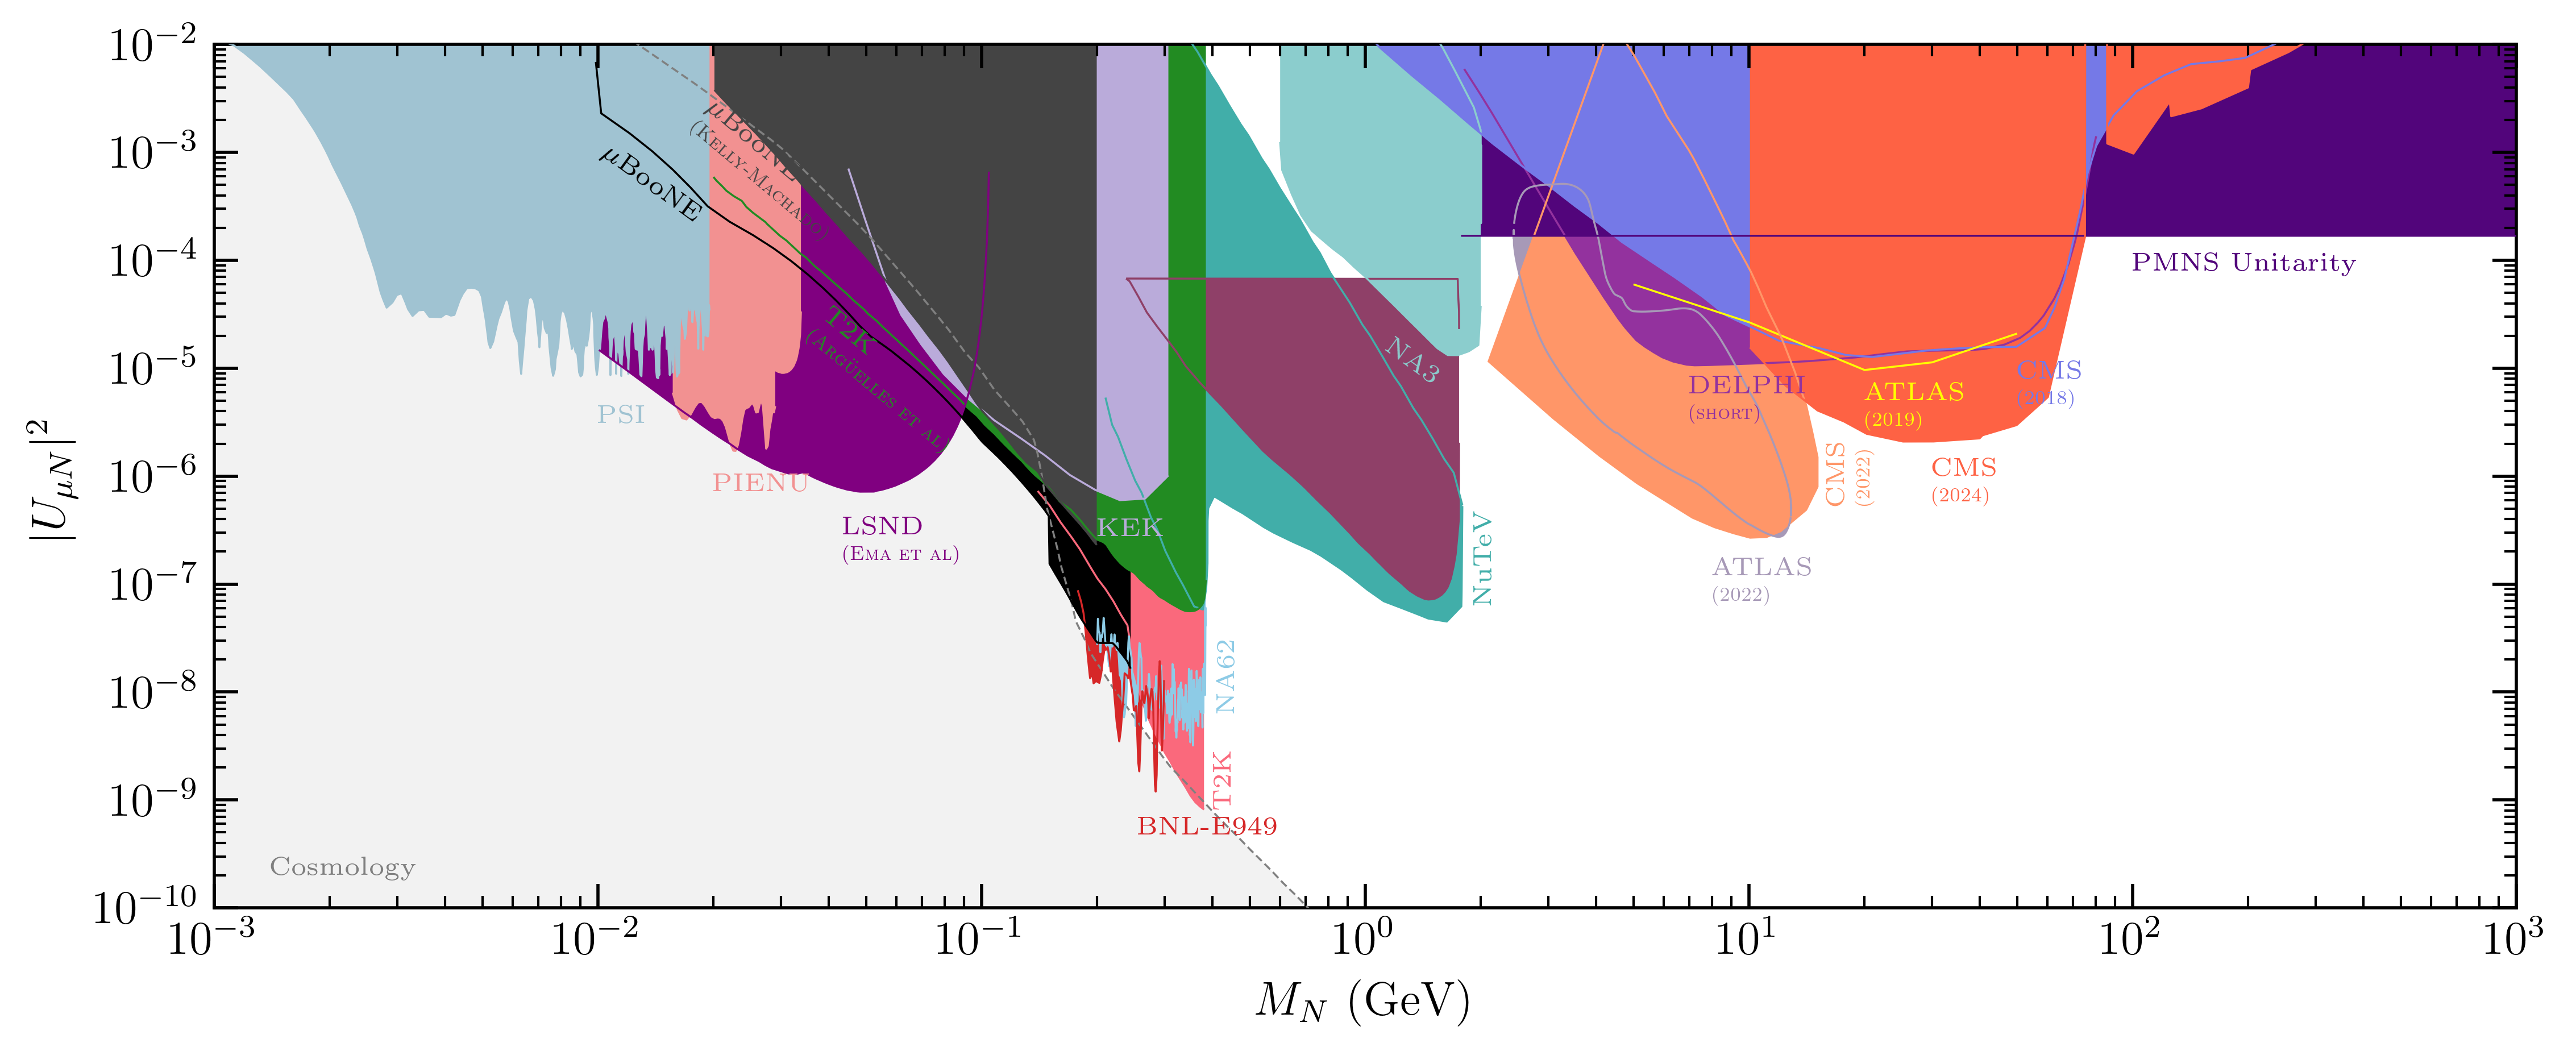
\includegraphics[width=1\linewidth]{figures/analysis_overview/HNL_summary_mu.png}
    \caption{Summary of exclusion limits imposed by various experiments on the square of the coupling of Heavy Neutral Leptons to the muon neutrino as a function of the HNL mass. The limits imposed by the ATLAS 2022 analysis is shown in grey as ATLAS (2022).~\cite{Fernandez-Martinez:2023phj}}
    \label{fig:HNL-summ-mu}
\end{figure}

\section{Dataset and Monte Carlo Simulations}\label{sec:data_mc_samples}
\subsection{ATLAS dataset}
The full Run-2 ATLAS dataset used for this analysis corresponds to an integrated luminosity of 140.1 $fb^{-1}$ of $pp$ collisions at $\sqrt{s}=$13~TeV. Only the subset of events satisfying the Good Run Lists are considered which have passed detector condition and data quality thresholds to ensure the data are suitable for physics analysis. The amount of data collected is roughly correlated to the pileup during a set period, since the collision rate is larger when a higher number of protons are squeezed together in a bunch.

The ATLAS data goes through a reconstruction chain as described in~\cref{sec:reco}, and is stored in a data format called Analysis Object Data (AOD). These files, due to the presence of low-level event information, are large in size and are designed to be used across ATLAS analyses. A further skimming is applied on these files based on specific analysis needs.
Given the non-standard nature of physics objects and reconstruction methods used in this analysis, a specialized data format, called DAOD\_LLP1, is used. This Derived AOD (DAOD) format adds information for a large breadth of analyses searching for LLPs which wouldn't be available in the standard DAOD formats. The secondary vertexing algorithm used in this analyses requires low-level track information which are available in the AODs but not in the DAODs, and hence is run at the AOD$\rightarrow$DAOD\_LLP1 step. 

\subsection{Simulated Samples}
The signal and background processes affecting this analysis are simulated using Monte Carlo (MC) event generation. These simulations start with the event generation of the underlying hard-scatter event along with the parton shower process. The simulation is followed by the modeling of the interaction of the particles with the active detector material done using the \textsc{Geant4}~\cite{AGOSTINELLI2003250} simulation toolkit. In the next step, additional $pp$ interactions are overlaid along with the hard-scatter according to the data taking conditions of a corresponding year, and the whole event goes through a digitization step where the detector readout response is simulated to represent the signature left by real particles in ATLAS. Three MC campaigns are simulated - mc20a, d, and e, corresponding to the pileup and detector conditions in the years 2015-16, 2017, and 2018, respectively. The simulated pileup profile is reweighted to match the total integrated luminosity of the data taking period. The digitized signature is reconstructed to build physics objects in the AOD format. Finally, DAOD\_LLP1 are created for both data and MC samplesto ensure the same treatment is applied to both.

\subsection*{Signal MC Samples}
Signal samples were generated using \textsc{MadGraph5\_aMC@NLO}~\cite{Alwall:2014hca} with HeavyN UFO model libraries~\cite{PhysRevD.94.053002} that provide a minimal extension to SM with Heavy Neutrinos at next-to-leading order QCD accuracy and uses the \textsc{NNPDF3.0nlo}~\cite{Ball:2014uwa} set of PDFs. The events were interfaced to \textsc{Pythia\,8.230}~\cite{Sjostrand:2014zea} to model the parton shower, hadronization, and underlying-event, with parameters set according to the A14 tune~\cite{ATL-PHYS-PUB-2014-021} and using the \textsc{NNPDF2.3nlo}~\cite{Ball:2012cx} set of PDFs.

The $W$ boson from the primary $pp$ interaction is required to decay into a muon or an electron, and a Heavy Neutral Lepton admixture ($W\to\ell\mathcal{N}$). The HNL is given a long lifetime and set to decay leptonically ($\mathcal{N}\to\ell\ell\nu$, $\ell=\mu$ or $e$, $\nu$ is the SM neutrino). The decay is modeled via a V-A weak matrix element, and can be mediated either via a virtual $W^*$ or $Z^*$. Both diagrams contribute to the decay if the charged leptons in the HNL decay have the same flavor.

Samples are created with mean decay lengths \ctau~= 1, 10, 100 mm and masses \mn~= 1, 2, 3, 4, 5, 7.5, 10, 12.5, 15, 17.5, 20 GeV. For masses up to 5 GeV, \ctau~= 1000 mm is also considered. Both lepton-number conserving and violating decays are simulated.

The various models considered in this analysis are summarized in~\cref{tab:hnl_models}. The simulated samples are scaled to different cross-sections based on the final state and the model being considered. Six decay modes are considered in this analysis determined by the flavor of the charged leptons. The channels are represented as $\ell_\alpha - \ell_\beta \ell_\gamma$, where $\alpha$ is the flavor of the prompt lepton, and $\beta$ and $\gamma$ are the flavors of the charged leptons from the HNL decay.~\Cref{tab:channels} summarizes the six final states considered in this analysis and the decay modes that lead to that final state. $\ell_\beta$ and $\ell_\gamma$ cannot be experimentally resolved and neutrinos flavors cannot be observed using the ATLAS detector. Hence, the $\ell_\beta\ell_\gamma\nu$ and $\ell_\gamma\ell_\beta\nu$ contributions are combined.


\begin{table}[!ht]
    \centering
    \begin{tabular}{cc|c}
        \hline\hline
         Final state/\ & \multicolumn{2}{c}{Decay mode from model with} \\
         Channel & Single flavor mixing HNL &  $\mu-$ and $e-$ mixing HNL \\
         \hline
         \uuu & $W\to\mu\mathcal{N}\left(\to\mu\mu\nu_\mu\right)$  & $W\to\mu\mathcal{N}\left(\to\mu\mu\nu_\mu + \mu\mu\nu_e \right)$\\
         \uue & $W\to\mu\mathcal{N}\left(\to\mu e\nu_e\right)$ & $W\to\mu\mathcal{N}\left(\to\mu e\nu_e + e\mu\nu_\mu \right)$\\
         \uee & $W\to\mu\mathcal{N}\left(\to e e\nu_\mu\right)$ & $W\to\mu\mathcal{N}\left(\to e e\nu_\mu + e e\nu_e\right)$\\
         \eee & $W\to e\mathcal{N}\left(\to e e \nu_e\right)$ & $W\to e\mathcal{N}\left(\to e e \nu_e +  e e \nu_\mu\right)$\\
         \eeu & $W\to e\mathcal{N}\left(\to e \mu\nu_\mu\right)$ & $W\to e\mathcal{N}\left(\to e \mu\nu_\mu + \mu e\nu_e\right)$\\
         \euu & $W\to e\mathcal{N}\left(\to\mu\mu\nu_e\right)$ & $W\to e\mathcal{N}\left(\to\mu\mu\nu_e + \mu\mu\nu_\mu\right)$\\
         \hline\hline
    \end{tabular}
    \caption{The six final states considered in this analysis and the decay modes that contribute to them for the different mixing models considered.}
    \label{tab:channels}
\end{table}

\subsection{Background MC Samples}
MC simulations are used to model the kinematics of the correlated background from SM processes contaminating the phase space explored in this analysis. Specifically, simulations of the top-quark pair production ($t\bar{t}$) and $V+$jets ($V=W,\xspace Z$) processes are considered.

The production of $t\bar{t}$ events was modelled using the \textsc{Powheg\,Box\,v2}~\cite{Frixione:2007nw,Nason:2004rx,Frixione:2007vw,Alioli:2010xd} generator at next-to-leading order with the \textsc{NNPDF3.0nlo}~\cite{Ball:2014uwa} PDF set and the \hdamp~parameter\footnote{The \hdamp~parameter is a resummation damping factor and one of the parameters that controls the matching of \textsc{Powheg} matrix elements to the parton shower and thus effectively regulates the high-\pT radiation against which the $t\bar{t}$ system recoils.} set to 1.5\,$m_{\mathrm{top}}$~\cite{ATL-PHYS-PUB-2016-020}.  The events were interfaced to \textsc{Pythia\,8.230}~\cite{Sjostrand:2014zea} to model the parton shower, hadronisation, and underlying event, with parameters set according to the A14 tune~\cite{ATL-PHYS-PUB-2014-021} and using the \textsc{NNPDF2.3lo} set of PDFs~\cite{Ball:2012cx}. The decays of bottom and charm hadrons were performed by \textsc{EvtGen\,1.6.0}~\cite{Lange:2001uf}. The non-all-hadronic slice of the sample is used, which includes leptonic final states.

The $W(\rightarrow \ell\nu)+$jets and $Z(\rightarrow \ell\ell)+$jets samples are generated using \textsc{Sherpa2.2.11}~\cite{Gleisberg:2008ta,Hoeche:2009rj,Bothmann:2019yzt} at next-to-leading order accuracy up to 2 jets, and up to leading order accuracy for up to 5 jets in the Matrix Element. The samples are created in three slices of the flavor of the jets, namely BFilter, CFilterBVeto, and CVetoBVeto, where XFilterYVeto refers to samples where a jet with flavor X is required and a jet with flavor Y is vetoed. Furthermore, for $\tau$ final states, the samples are divided by the decays of the $\tau$ lepton as either leptonic or (semi-)hadronic. For the predictions used in this analysis, all the slices and filters are combined for the total expected event yield.
 
\subsection{Signal Kinematics}
The position of the HNL decay depends on its proper lifetime and its boost, and the kinematics of its decay products depend on its mass and its boost.~\Cref{fig:truth_kinematics} shows some representative kinematic distributions of the HNL and its decay products at the \textit{truth level}, i.e. the actual kinematics of the simulated particles inside the ATLAS experiment. Such distributions are typically contrasted against kinematics at the \textit{reconstructed level}, i.e. kinematics of the particles after digitization, reconstruction, and identification of the same simulated particles.

\begin{figure}[!ht]
    \centering
     \subfloat[HNL decay radius]{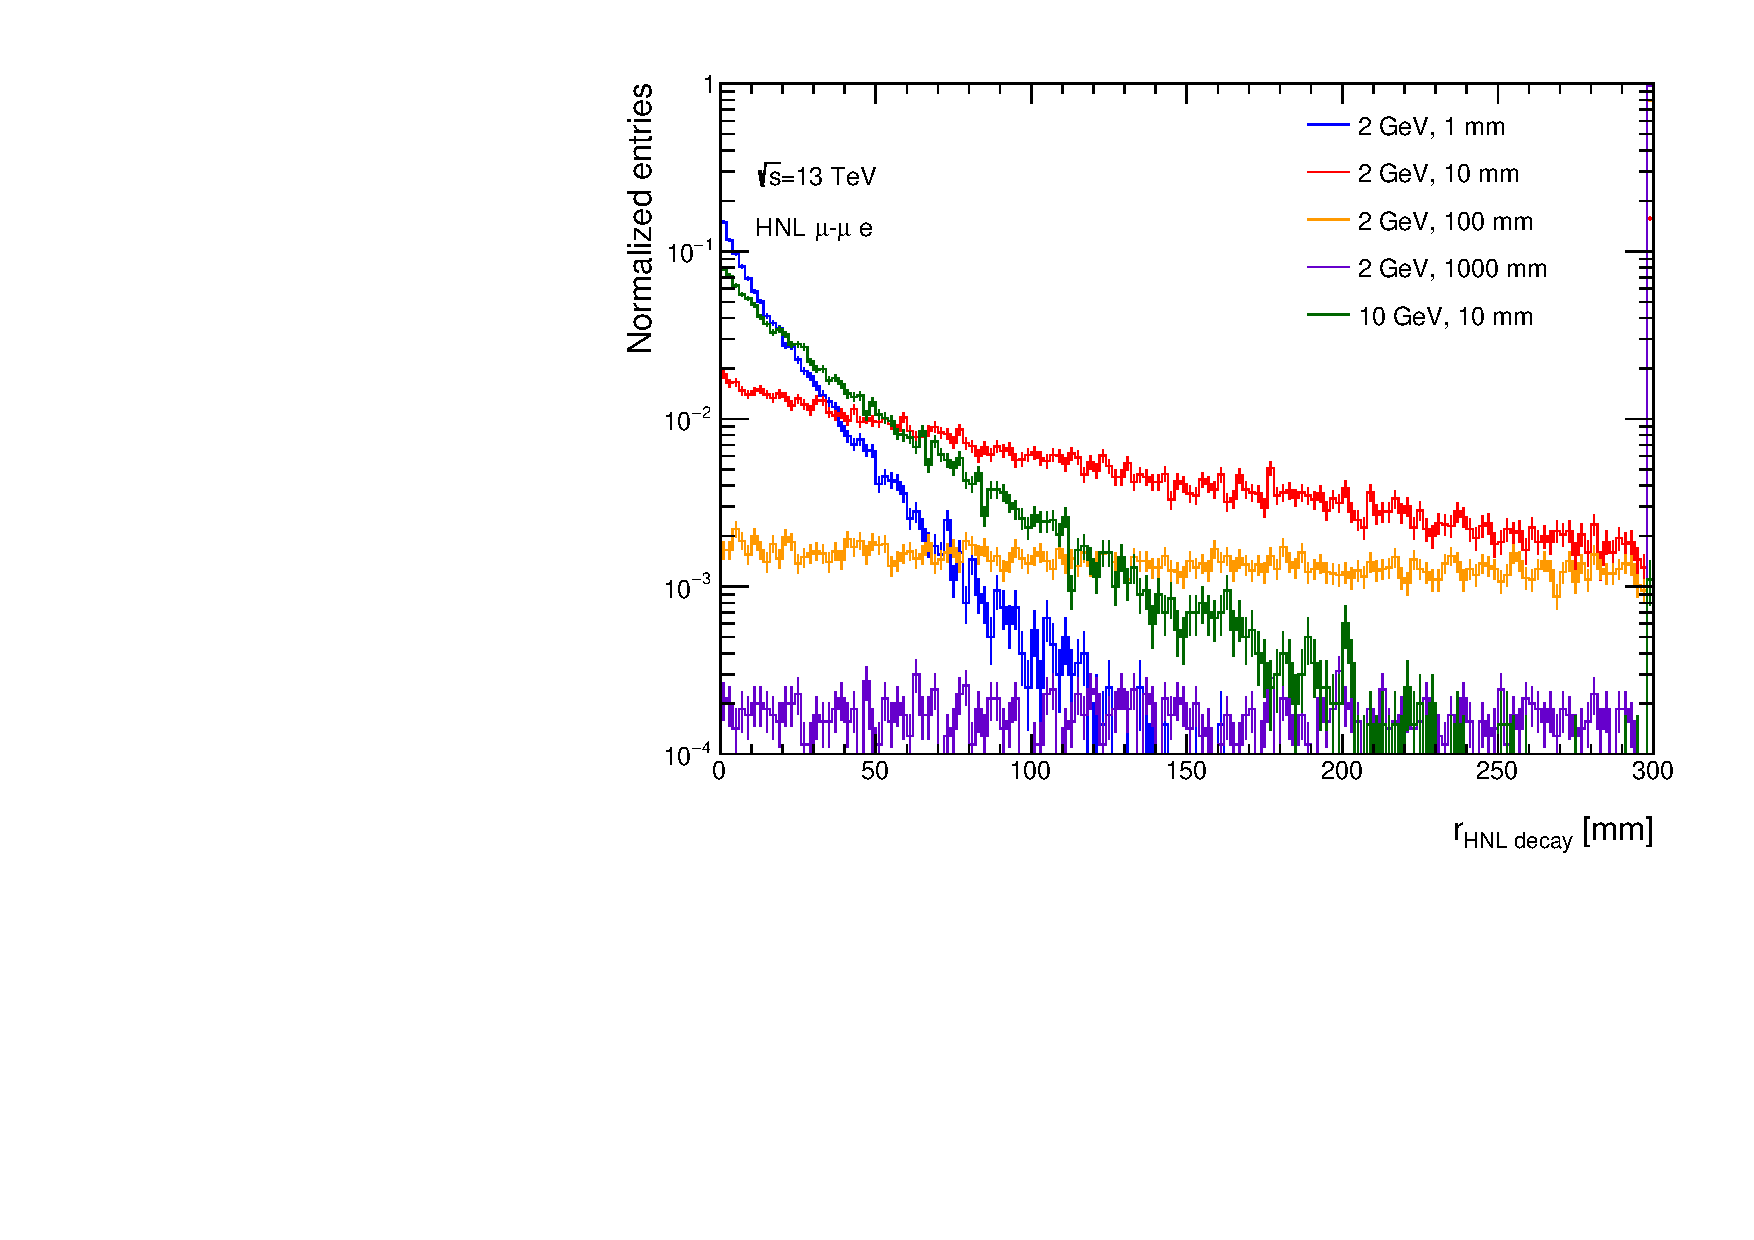
\includegraphics[width=0.45\textwidth]{figures/analysis_overview/TruthKinematics/rProd.pdf}\label{fig:kinem_rprod}}
     \subfloat[$\mu$ or $e$ $|d_0|$ ]{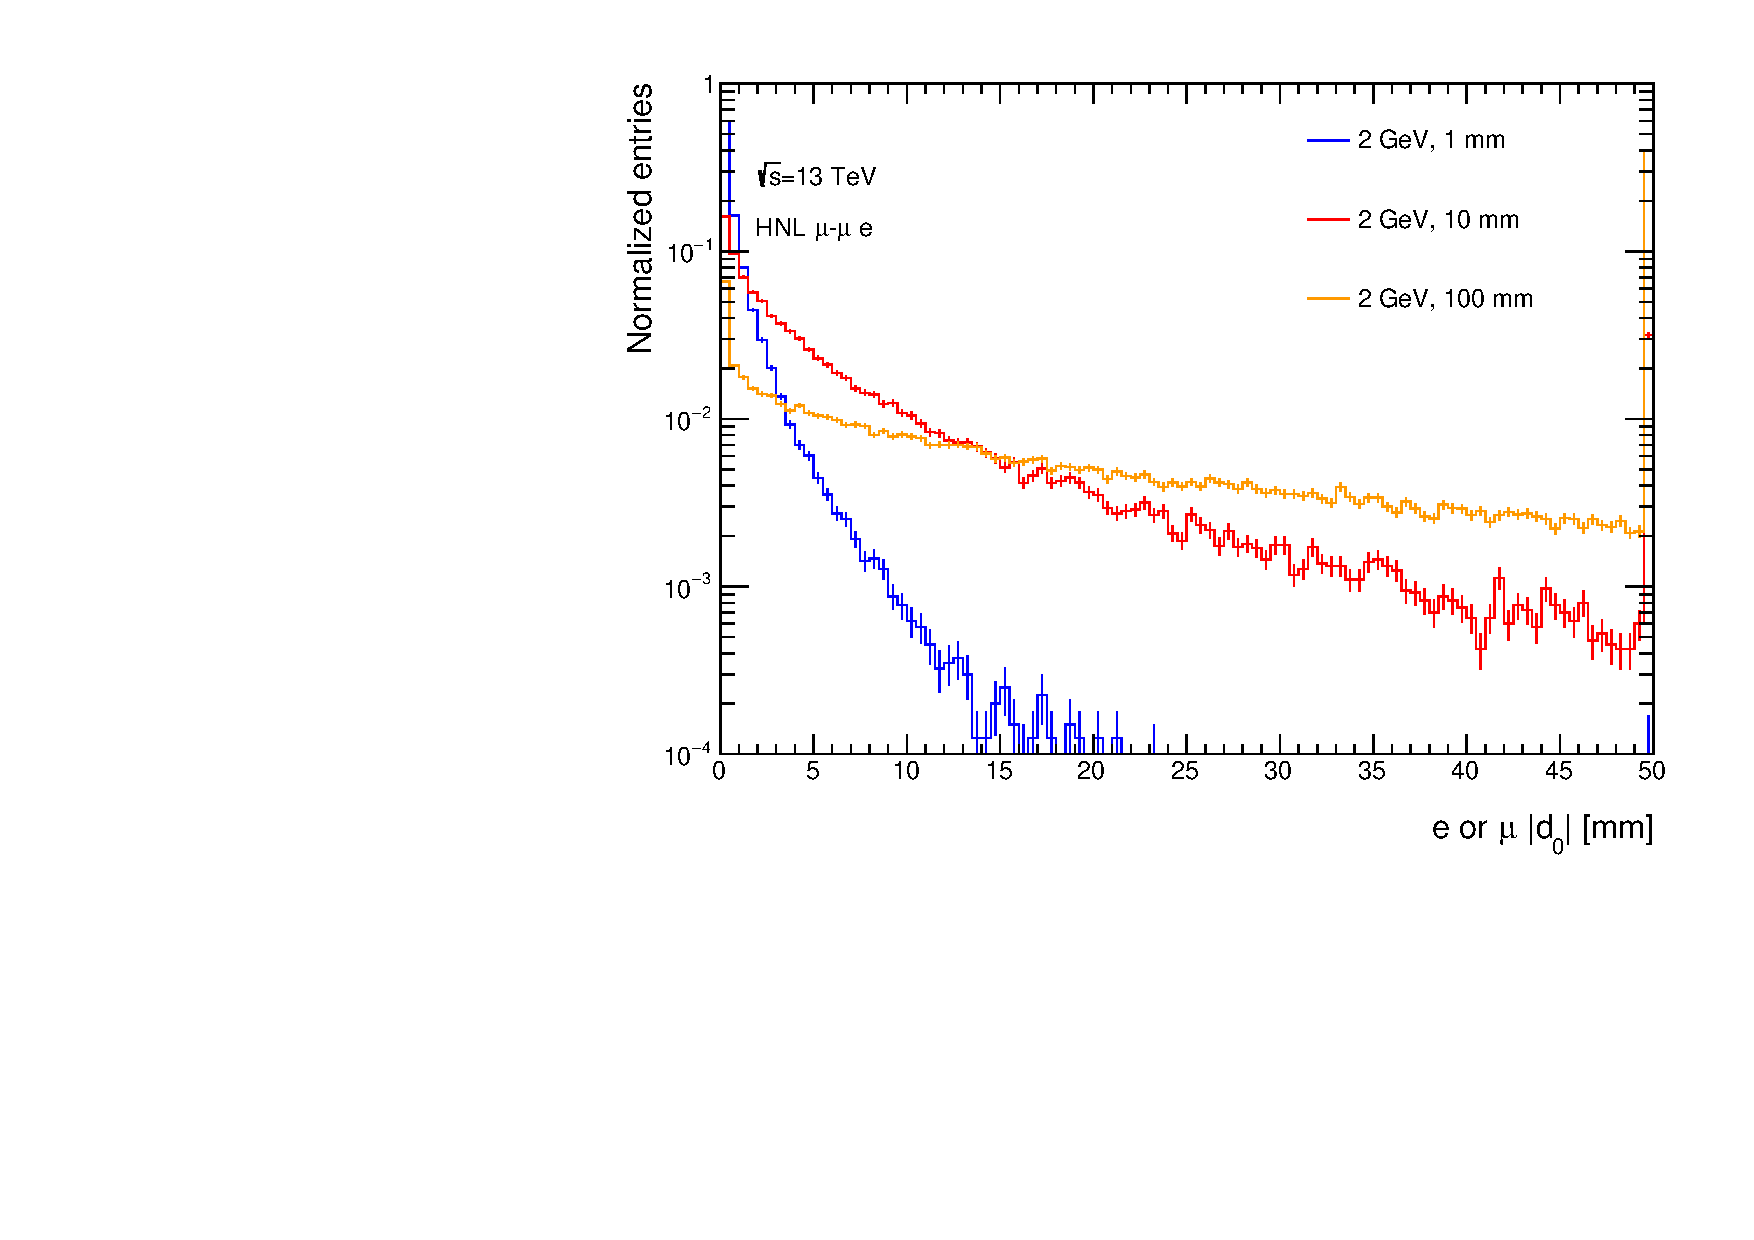
\includegraphics[width=0.45\textwidth]{figures/analysis_overview/TruthKinematics/lepD0.pdf}\label{fig:kinem_d0}} \\
     \subfloat[$\mu$ or $e$ \pT]{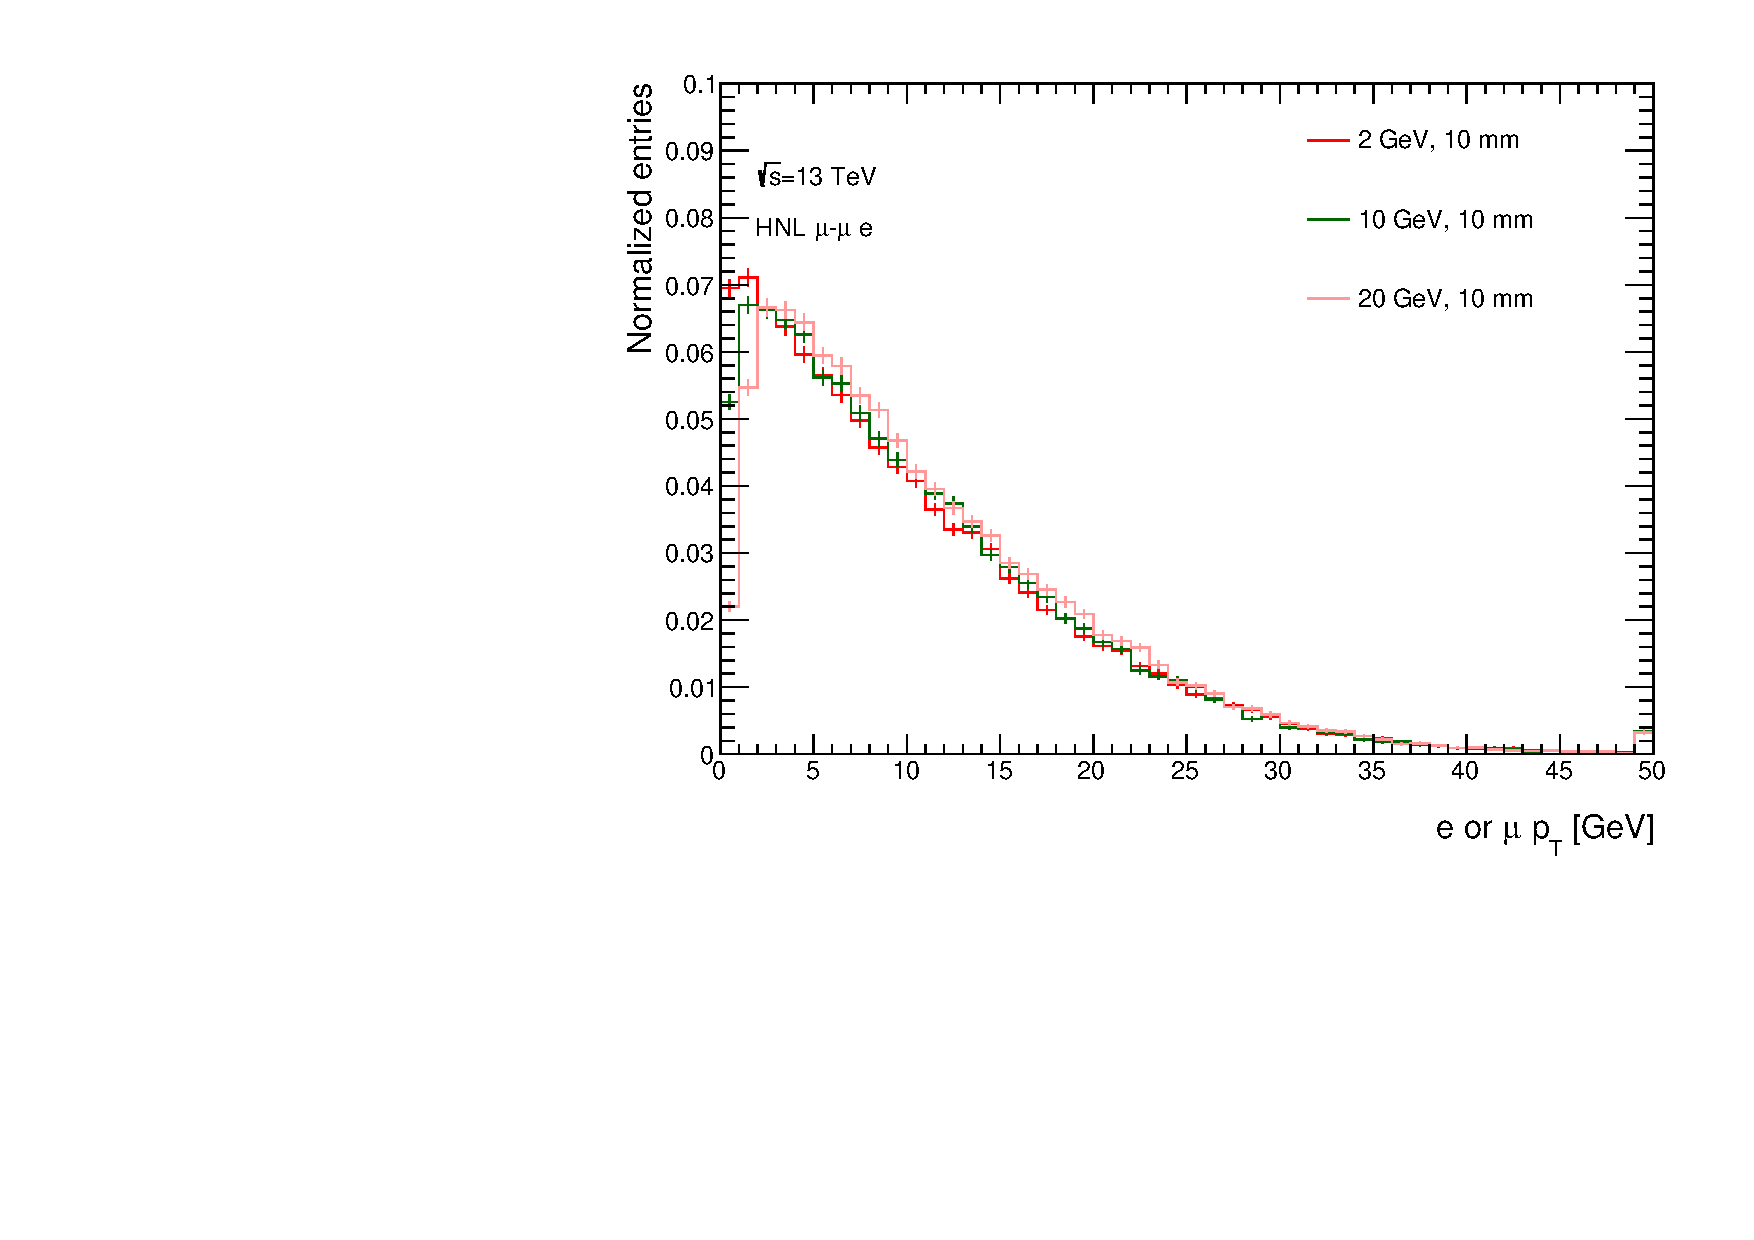
\includegraphics[width=0.45\textwidth]{figures/analysis_overview/TruthKinematics/lepPt.pdf}\label{fig:kinem_pt}}
     \subfloat[$\mu$ or $e$ $\eta$]{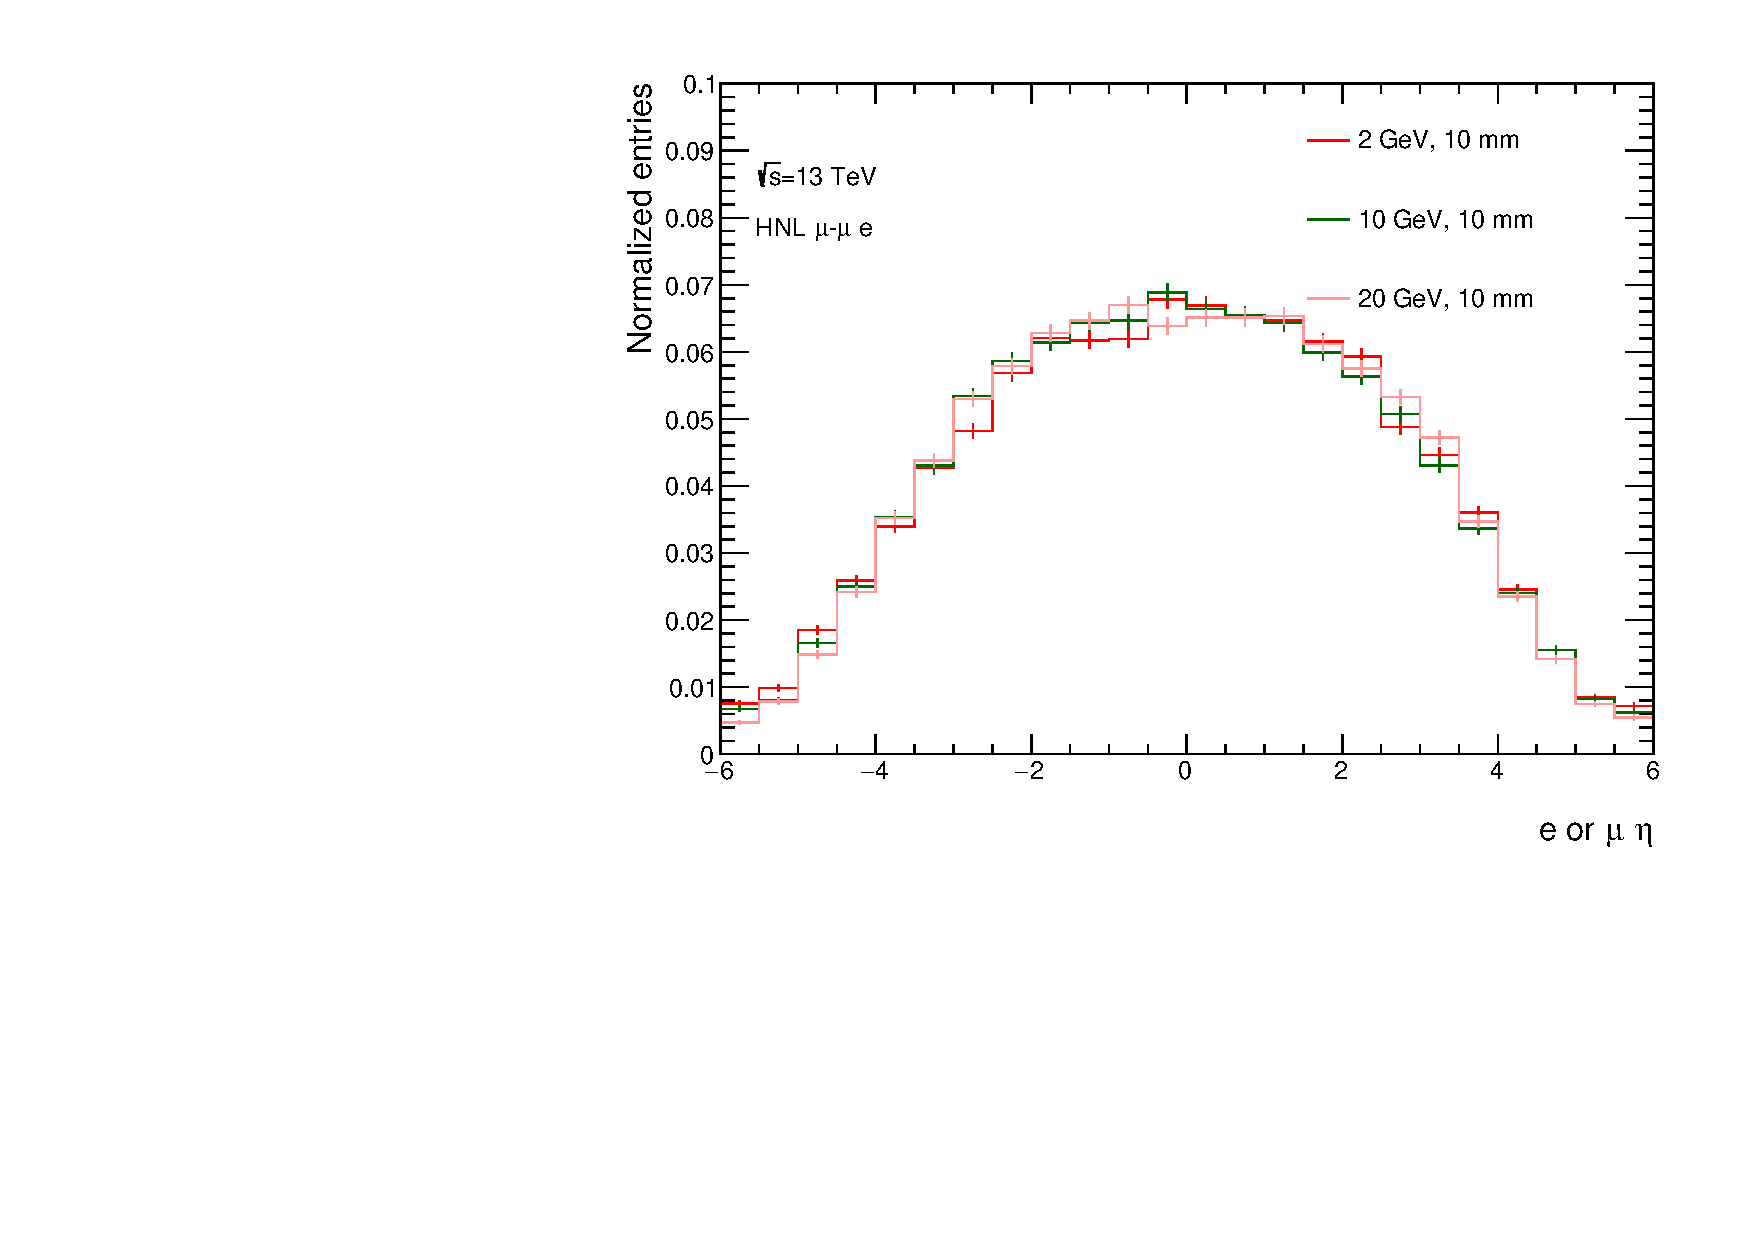
\includegraphics[width=0.45\textwidth]{figures/analysis_overview/TruthKinematics/lepEta.pdf}\label{fig:kinem_eta}}
     \caption{Truth level kinematic distributions for \uue HNL samples for some representative masses and proper lifetimes indicated in the legend. The total entries for each histogram are normalized to 1 for a fair comparison comparison, and overflow (underflow) is shifted into the first (last) bin.}
     \label{fig:truth_kinematics}
 \end{figure}

In the frame of the HNL, the probability density for it to decay is given by the exponential distribution:
\begin{equation}
    p_\mathrm{decay}(t)=e^{-t/\tau_\mathcal{N}}.
\end{equation}
In the lab frame, the radial position of the HNL decay, as illustrated in~\cref{fig:kinem_rprod}, depends on both its mass and proper lifetime due to a time dilation effect from its Lorentz boost. The track reconstruction efficiency drops after 300 mm due to the lack of enough silicon hits in the ID, causing most of the HNL decays for \ctau = 100 mm and 1000 mm to lie outside acceptance.~\Cref{fig:kinem_d0} shows the $|d_0|$ distribution for the charged decay products of the HNL which is independent of the mass of the HNL for a fixed proper lifetime. LRT adds sensitivity to higher lifetime HNLs since they have a large proportion of decays with $|d_0|>5\,$mm.~\Cref{fig:kinem_pt,fig:kinem_eta} show that the \pT and $\eta$ spectrum of the HNL decay products have a weak dependency on the mass and the lifetime being considered, especially in the \mhnl$<<m_W$ regime, where most of the momentum from the $W$ decay is transferred to the prompt lepton.

After studying the truth-level kinematics of the HNL signal, the simulated samples are used to quantify the detector acceptance and reconstruction efficiencies of the HNL samples as shown in~\cref{fig:acc_and_eff}.

\begin{figure}[!ht]
    \centering
     \subfloat[Acceptance Categorization]{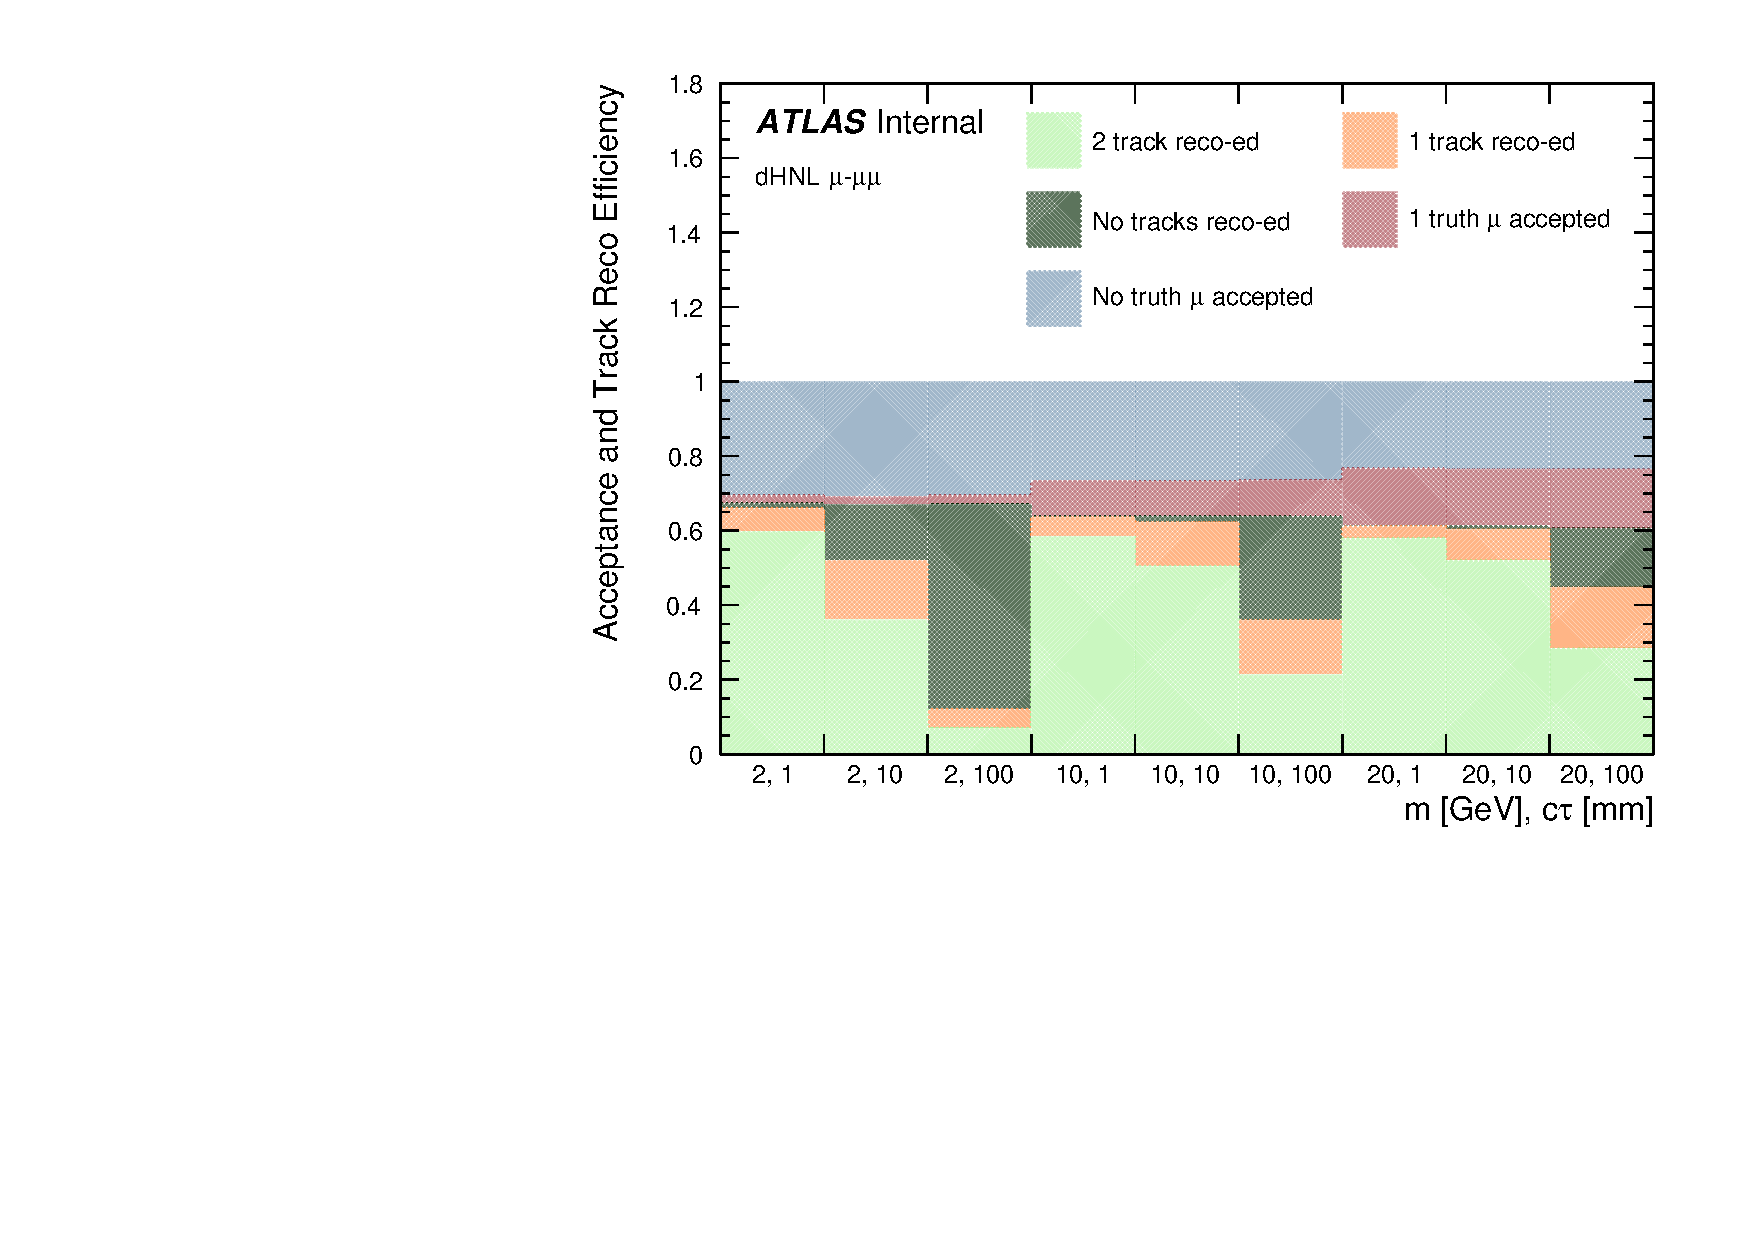
\includegraphics[width=0.45\textwidth]{figures/analysis_overview/TruthKinematics/plots_truth_eff_stack.pdf}\label{fig:categ_truth}}
     \subfloat[Reconstruction Categorization]{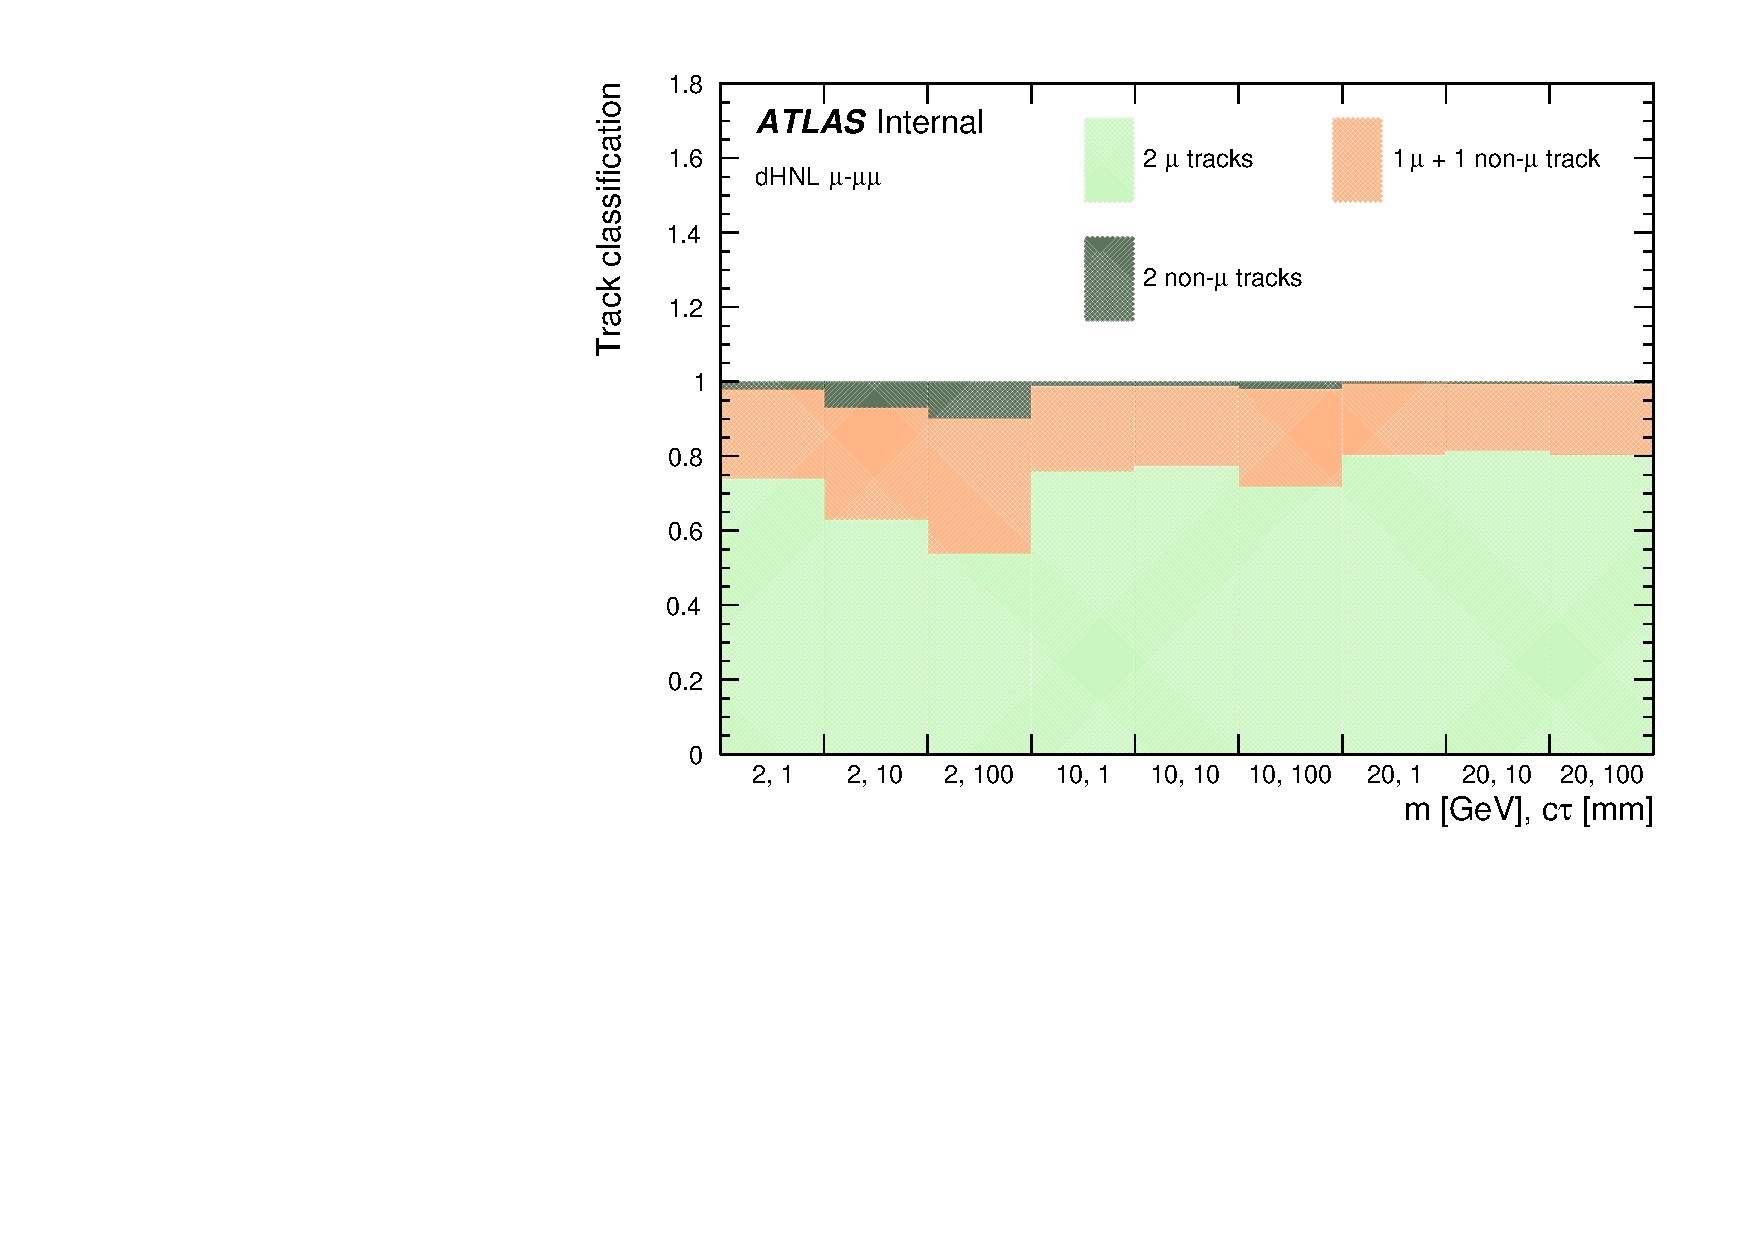
\includegraphics[width=0.45\textwidth]{figures/analysis_overview/TruthKinematics/plots_reco_eff_stack.pdf}\label{fig:categ_reco}}
     \caption{Fractional detector acceptance, ID track reconstruction, and muon reconstruction efficiencies for \uuu HNL samples for some representative mass and proper lifetimes indicated on the $x-$axis.}
     \label{fig:acc_and_eff}
 \end{figure}

~\Cref{fig:categ_truth} classifies HNL di-muon decays according to the detector and kinematic acceptance (\pT$>3$~GeV, $|\eta|<2.7$) of a truth muon and if the truth muon leaves hits that are reconstructed as an ID track. The fraction of events where both muons are reconstructed as tracks is within 5-60\% with a strong dependence on the HNL proper lifetime and a weak dependence on its mass, since they affect the production radius of the muons and hence their tracking acceptance.~\Cref{fig:categ_reco} further categorizes the cases with two reconstructed ID tracks according to their muon extension efficiency i.e. if the ID tracks are matched to reconstructed muons. A stronger (yet still subtle in the masses considered) dependency is observed on the HNL mass than lifetime, since the \pT spectrum of the muons are skewed towards higher values for heavier HNLs, as shown in~\cref{fig:kinem_pt}. Hence, low mass and high lifetime HNLs suffer from low detector acceptance and low lepton reconstruction efficiencies. This fact, further convoluted with the low cross-section of HNL production in that phase space, makes the exploration of lighter and weakly-coupled HNLs extremely challenging.

\section{Physics Objects Selection}\label{sec:object_sel}
The final state probed in this analysis is characterized by a prompt lepton and a displaced vertex in the ID volume with two outgoing leptons. Furthermore, some requirements on the quark flavor of jets in the event are imposed in the definition of analysis regions.

\subsection{Prompt Lepton and Trigger}
A prompt lepton is defined as a muon or an electron coming from the primary $pp$ interaction. The prompt lepton is used as the primary triggering object to tag the $W$-decay, and hence, the requirements on the selection of the prompt lepton are driven by the selections imposed by the trigger chain. The identification Working Point (WP) adds self-consistency and goodness of fit requirements on the lepton object to select genuine leptons against incorrect combinations of hits or hadron decays-in-flight. Similarly, isolation separates leptons without hadronic or radiative activity around them from those that are within jets. Finally, track-to-vertex association applies cuts so that the lepton points back to the primary $pp$ collision.~\Cref{tab:plep_selection} summarizes the selections imposed on the prompt lepton candidate.

\begin{table}[!ht]
    \centering\small
    \begin{tabular}{cc}
        \hline\hline
        Cut Name & Cut Description \\
        \hline
        Lepton Flavor & muon or electron \\
        Trigger Matched & $\checkmark$ \\
        Transverse Momentum & \pT $>$ 27 GeV \\
        Identification Working Point & \texttt{Medium}~\cite{MUON-2018-03,PERF-2017-01} \\
        Isolation Working Point & \texttt{PflowLoose\_VarRad}~\cite{MUON-2018-03} (\texttt{Loose\_VarRad}~\cite{EGAM-2018-01}) for $\mu\,(e)$ \\
        Track-to-Vertex-Association & $|d_{0}/\sigma(d_{0})| < 3\,(5)$ for $\mu\,(e)$, $|z_{0}\sin{\theta}| < 0.5$ mm~\cite{MUON-2018-03,EGAM-2018-01} \\
        \hline\hline
    \end{tabular}
    \caption{Selections used for the prompt lepton candidate.}
    \label{tab:plep_selection}
\end{table}

If more than one prompt lepton candidate are found in an event, the candidate with the highest transverse momentum is chosen as the prompt lepton.

\begin{table}[!ht]
    \centering\small
    \begin{tabular}{ccc}
        \hline\hline
        Period & Muon Trigger & Electron Trigger \\
        \hline
        2015 & HLT\_mu20\_iloose\_L1MU15 & HLT\_e24\_lhmedium\_L1EM20VH \\
        2016, 2017, 2018 & HLT\_mu26\_ivarmedium & HLT\_e26\_lhtight\_nod0\_ivarloose \\
        \hline\hline
    \end{tabular}
    \caption{Lowest unprescaled single lepton triggers used in the analysis.}
    \label{tab:triggers}
\end{table}

\begin{figure}[!ht]
    \centering
     \subfloat[\uuu \mn=10 GeV]{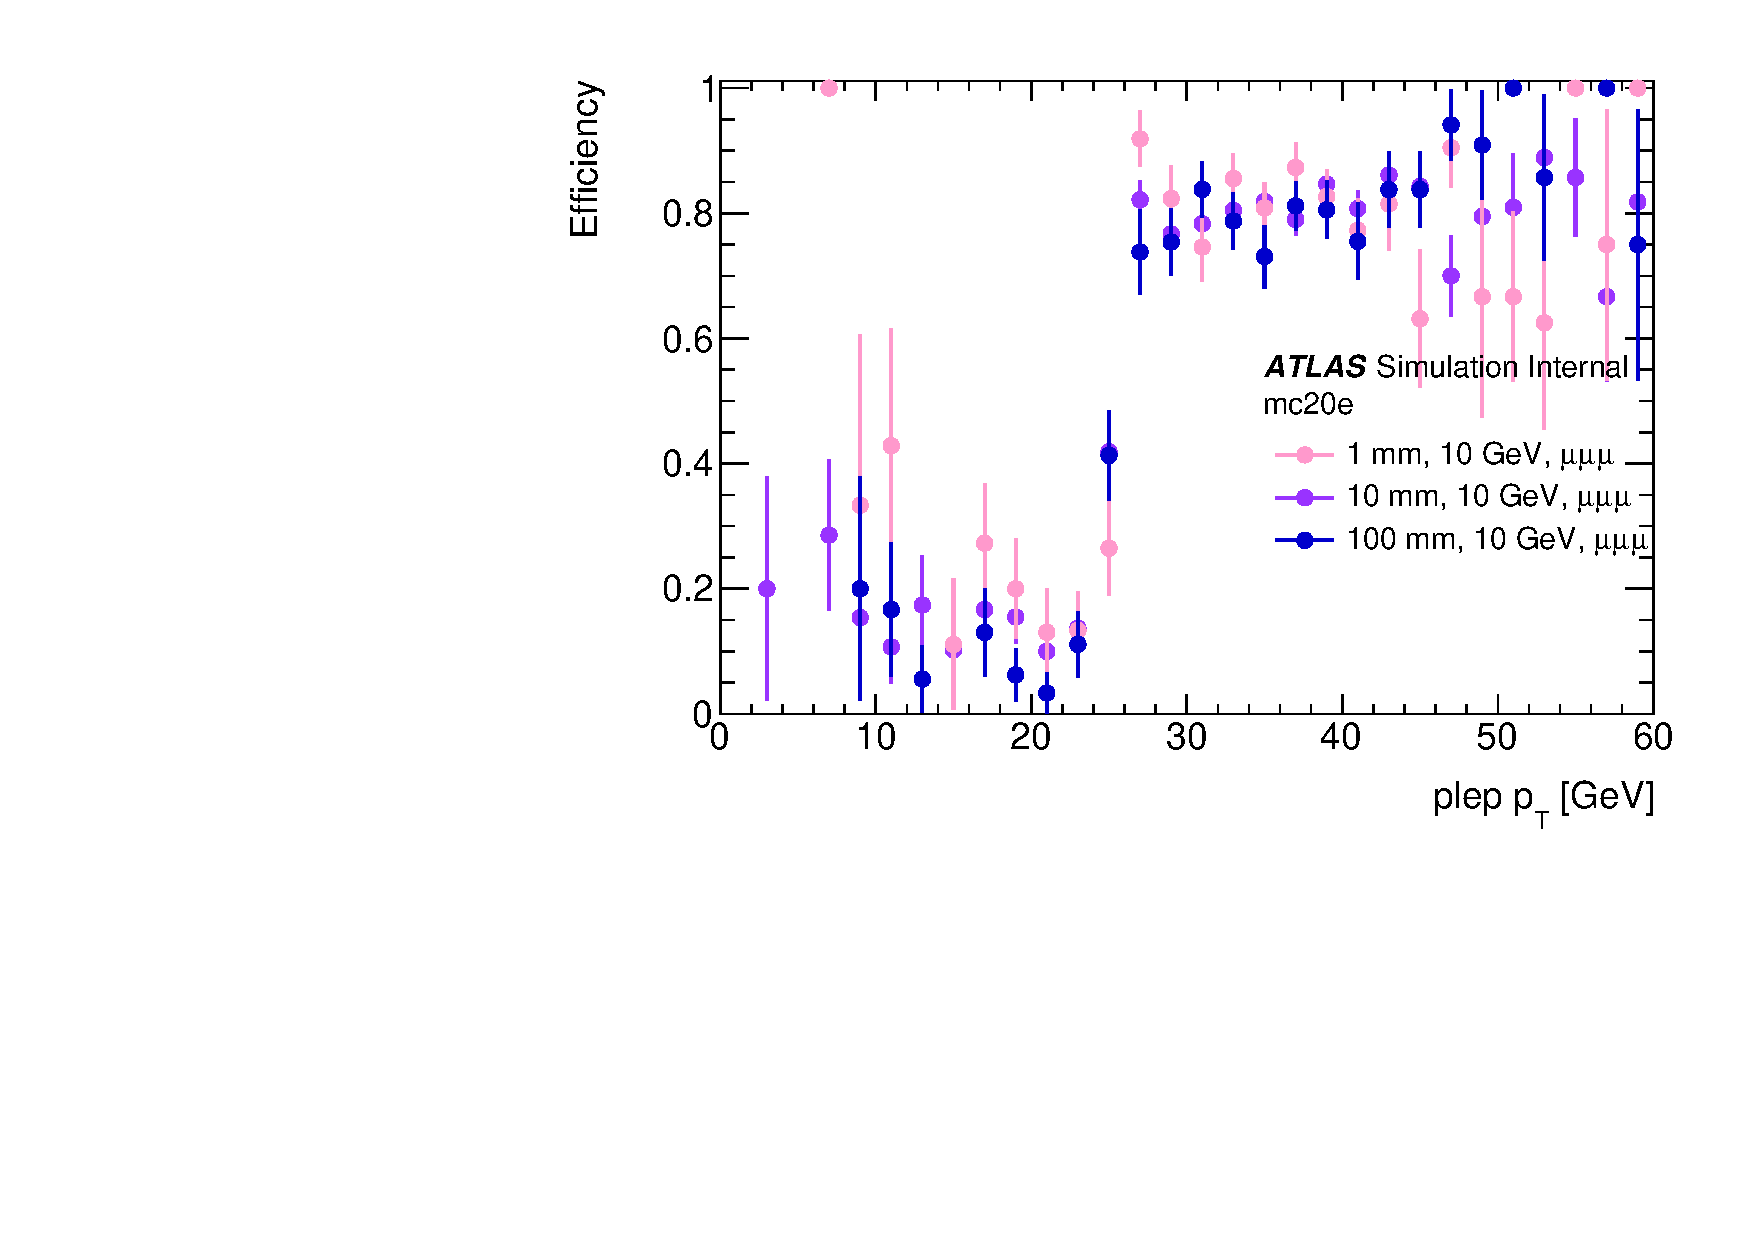
\includegraphics[width=0.45\textwidth]{figures/analysis_overview/trigger/effbylifetime_uuu.pdf}}
     \subfloat[\eee \mn=10 GeV]{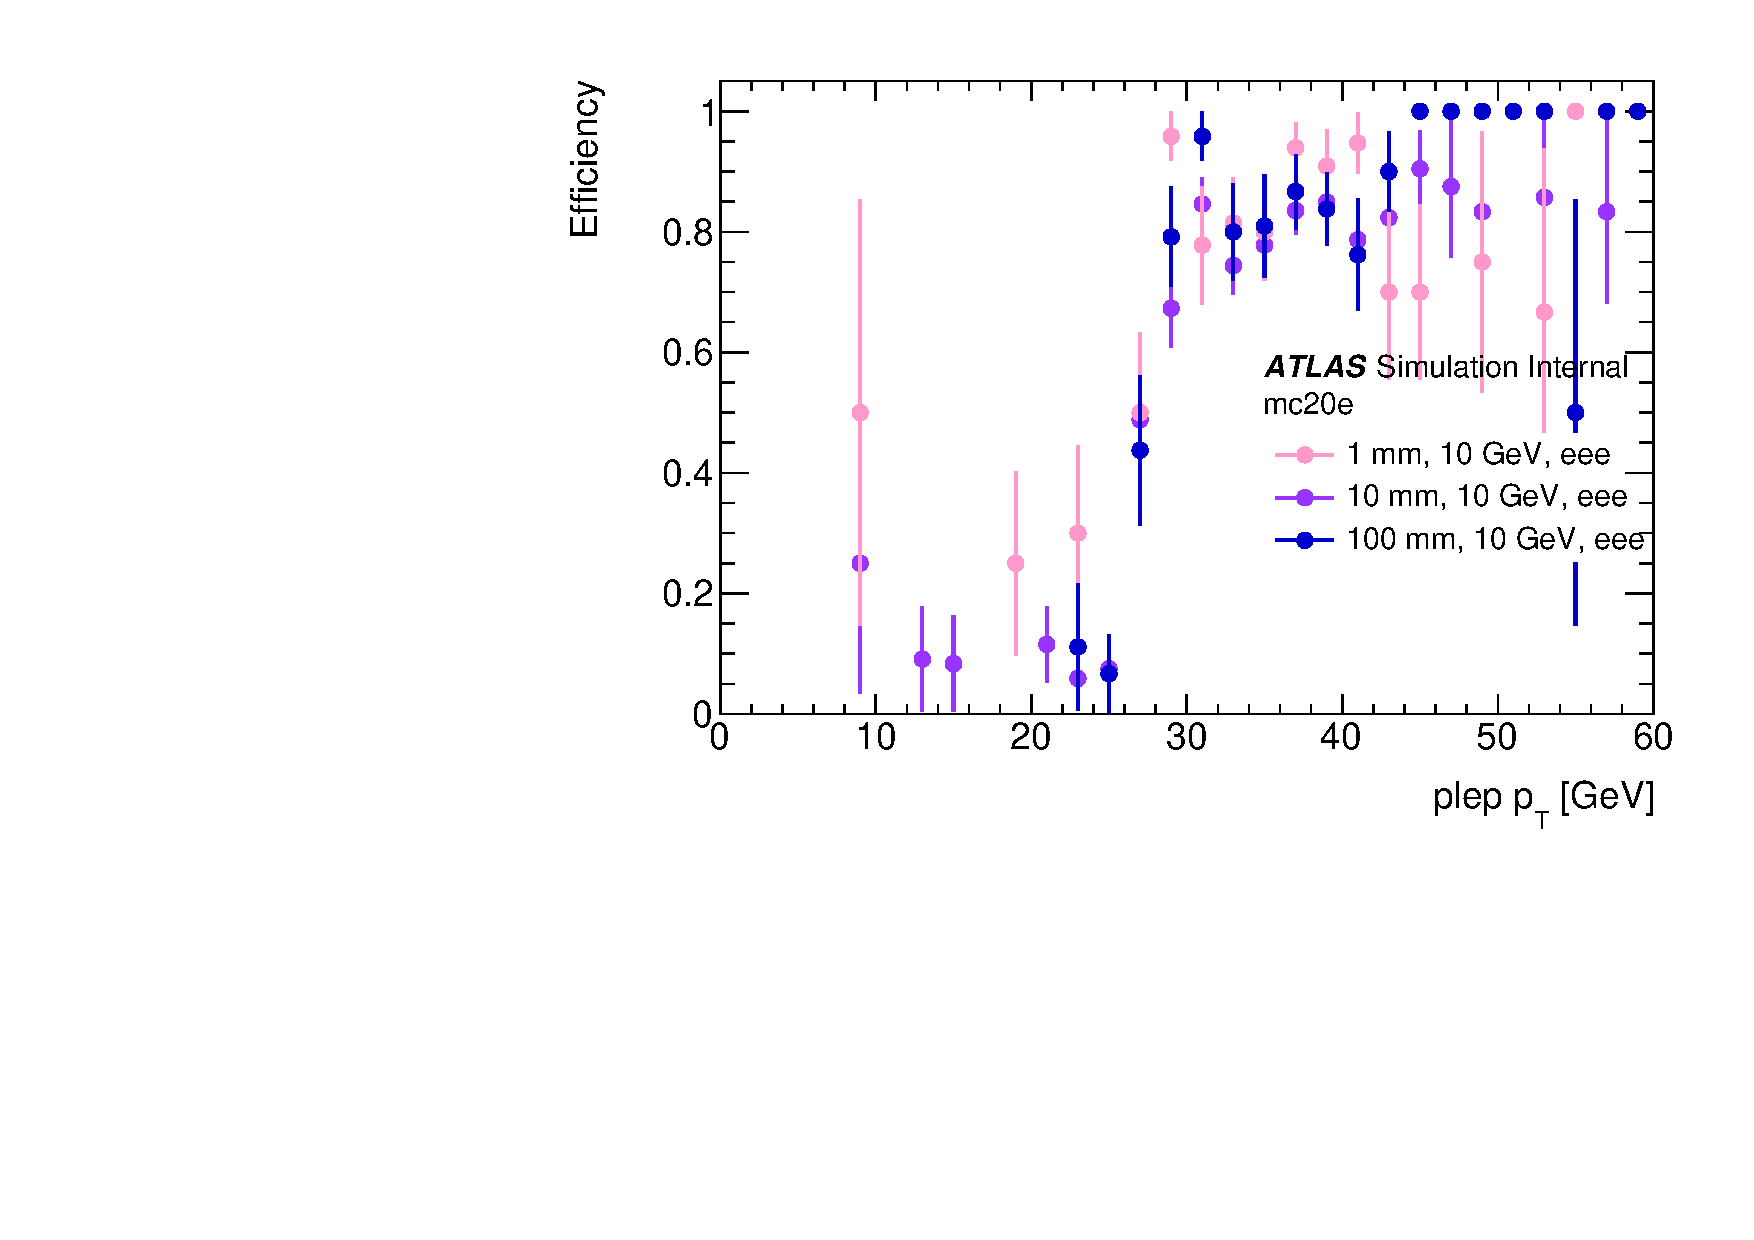
\includegraphics[width=0.45\textwidth]{figures/analysis_overview/trigger/effbylifetime_eee.pdf}} \\
     \subfloat[\uuu \ctau=10 mm]{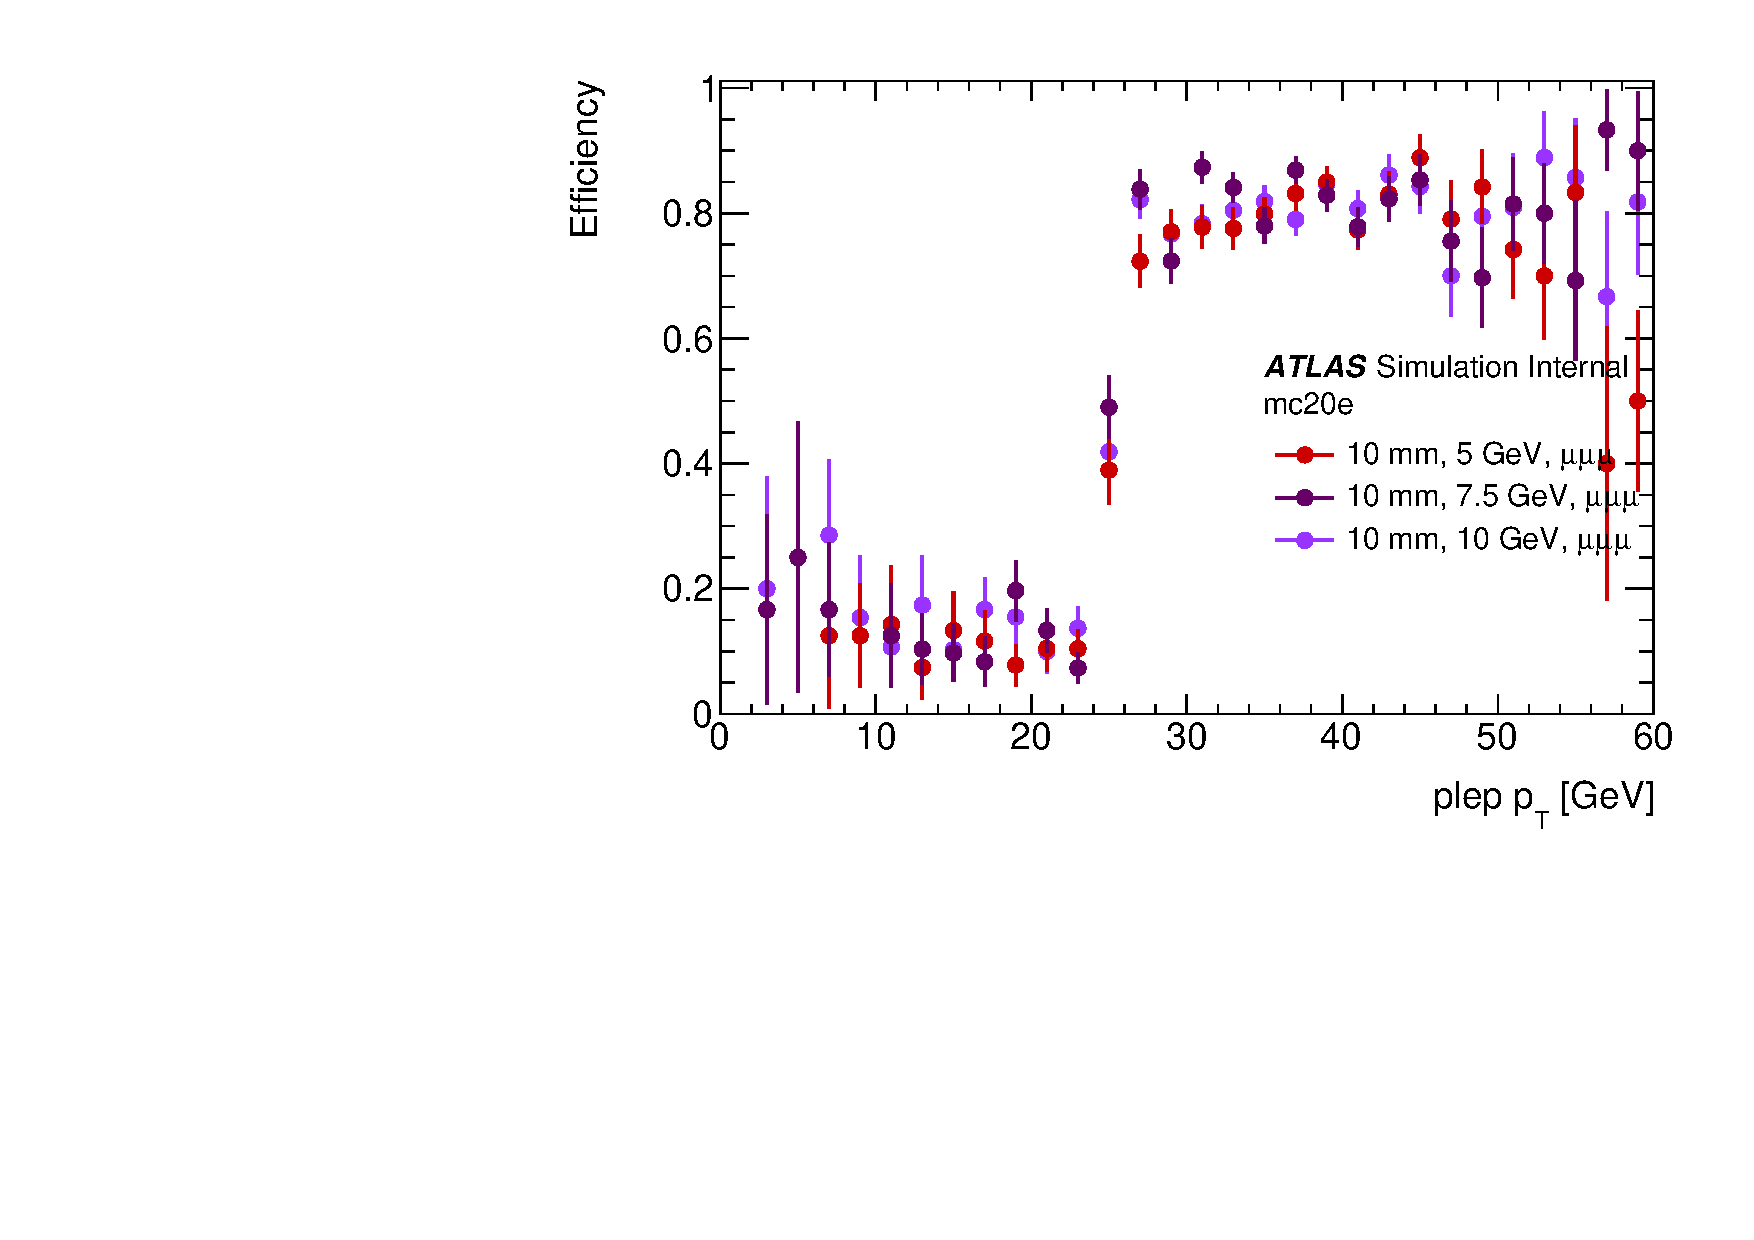
\includegraphics[width=0.45\textwidth]{figures/analysis_overview/trigger/effbymass_uuu.pdf}}
     \subfloat[\eee \ctau=10 mm]{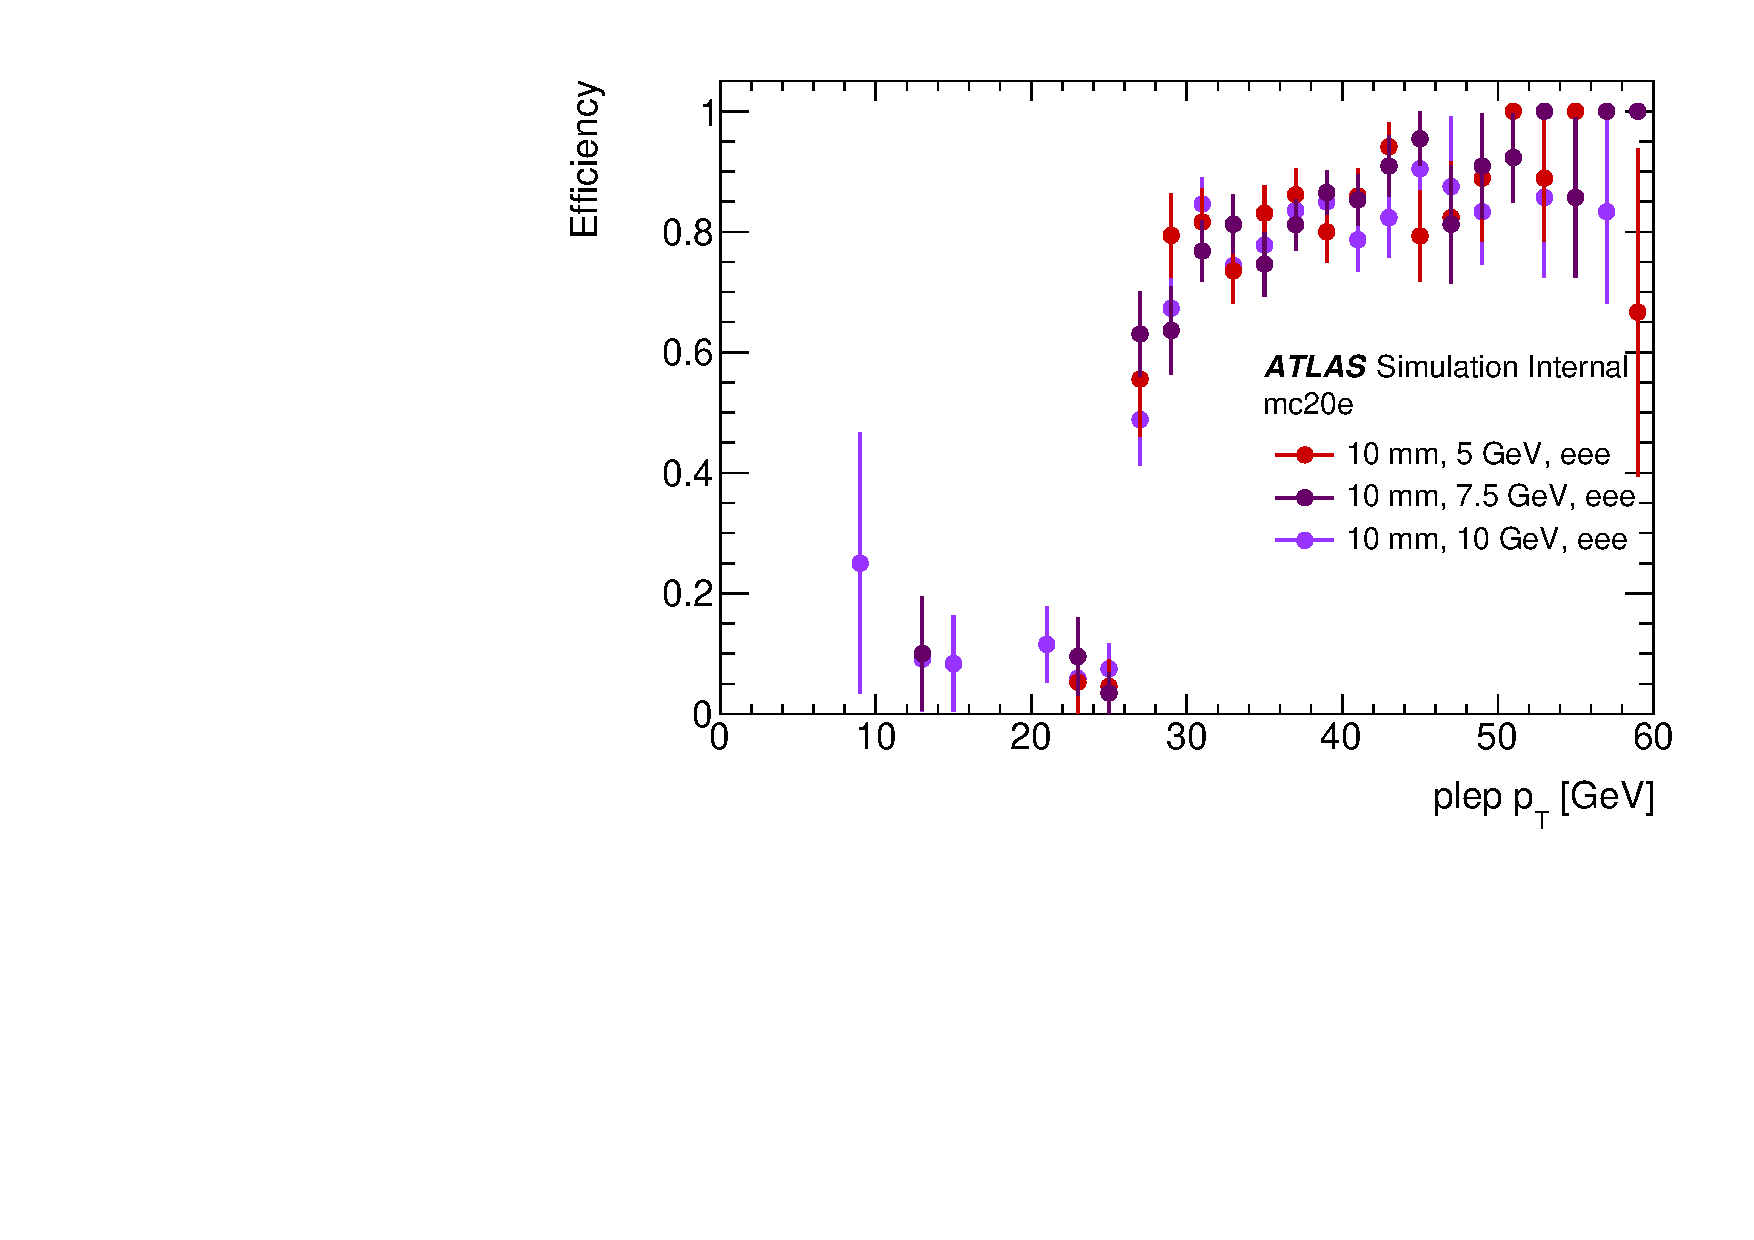
\includegraphics[width=0.45\textwidth]{figures/analysis_overview/trigger/effbymass_eee.pdf}}
     \caption{Fraction of events where any single-lepton trigger is fired by any lepton as a function of the prompt lepton \pT for a selection of HNL signal mass and lifetimes for the \uuu and \eee channels.}
     \label{fig:trigger_eff}
\end{figure}

The lowest unprescaled single lepton triggers are used in this analysis, with the exact trigger scheme for each data taking year listed in~\cref{tab:triggers}. ~\Cref{fig:trigger_eff} shows the fraction of events where a single lepton fires the trigger as a function of the prompt lepton \pT for the single muon and single electron triggers for a selection of \uuu and \eee signal samples. The low \pT tail on the plots come from events in which the lepton causing the trigger originated from the displaced leptons. This tail would disappear once the selections on the prompt lepton are applied. The selections in~\cref{fig:trigger_eff} are limited to the presence of a PV, a prompt lepton (without any selections), and the presence of a $\mu\mu$ or $ee$ DV in the fiducial volume.

\subsection{Displaced Muons}
Muons in the displaced vertex are referred to as displaced muons. Since these muons are produced from a decay away from the IP, they are not always expected to point back to it. Hence, to extend the analysis coverage to such non-pointing muons, a combination of standard and LRT muons are used.

As described in~\cref{sec:reco}, the standard (i.e. both primary and inside-out) muon reconstruction and LRT muon reconstruction run seperately using all the hits in the MS in an event as inputs along with the standard ID tracks for the former chain and the LRT tracks for the latter chain. This workflow, due to the use of all MS hits in both the chains, causes a large fraction of LRT muons to share MS hits (or rather a full MS track) with a standard muon. The LRT and standard muon are hence said to have an \textit{overlap} with each other. This is an unphysical situation since it's not possible for two genuine muons to leave identical MS hits. However, the muon reconstruction algorithm is very liberal in the quality of muons it reconstructs, and hence a bad quality LRT muon could overlap with a good quality standard muon, and vice versa. An overlap resolution strategy is designed to retain or reject a muon object from a pair (out of which one is reconstructed as a standard muon and the other as a LRT muon) which share an MS track between them. The strategy is optimized for maximal signal retention post overlap removal, and uses fundamental muon quality requirements without adding any biases from the kinematics of the signal. In case both or neither muon passes a check, the resolution moves on to the next check. The overlap resolution is designed to, in case of a MS track overlap, retain the muon which passes these requirements, followed sequentially:
\begin{itemize}
    \item passes the \texttt{Loose}~\cite{MUON-2018-03}\footnote{The \texttt{Loose} criteria used here is modified to not apply any requirements on the ID track.} identification working point,
    \item is a Combined muon,
    \item has a lower absolute $\eta$ difference between the measurement from ID track and the MS track extrapolated to the perigee,
    \item is reconstructed in the standard pass (fallback option).
\end{itemize}
~\Cref{fig:muon_overlap} shows the fraction of standard and LRT muons which have an overlap at different stages of the overlap removal process.

\begin{figure}[!ht]
    \centering
    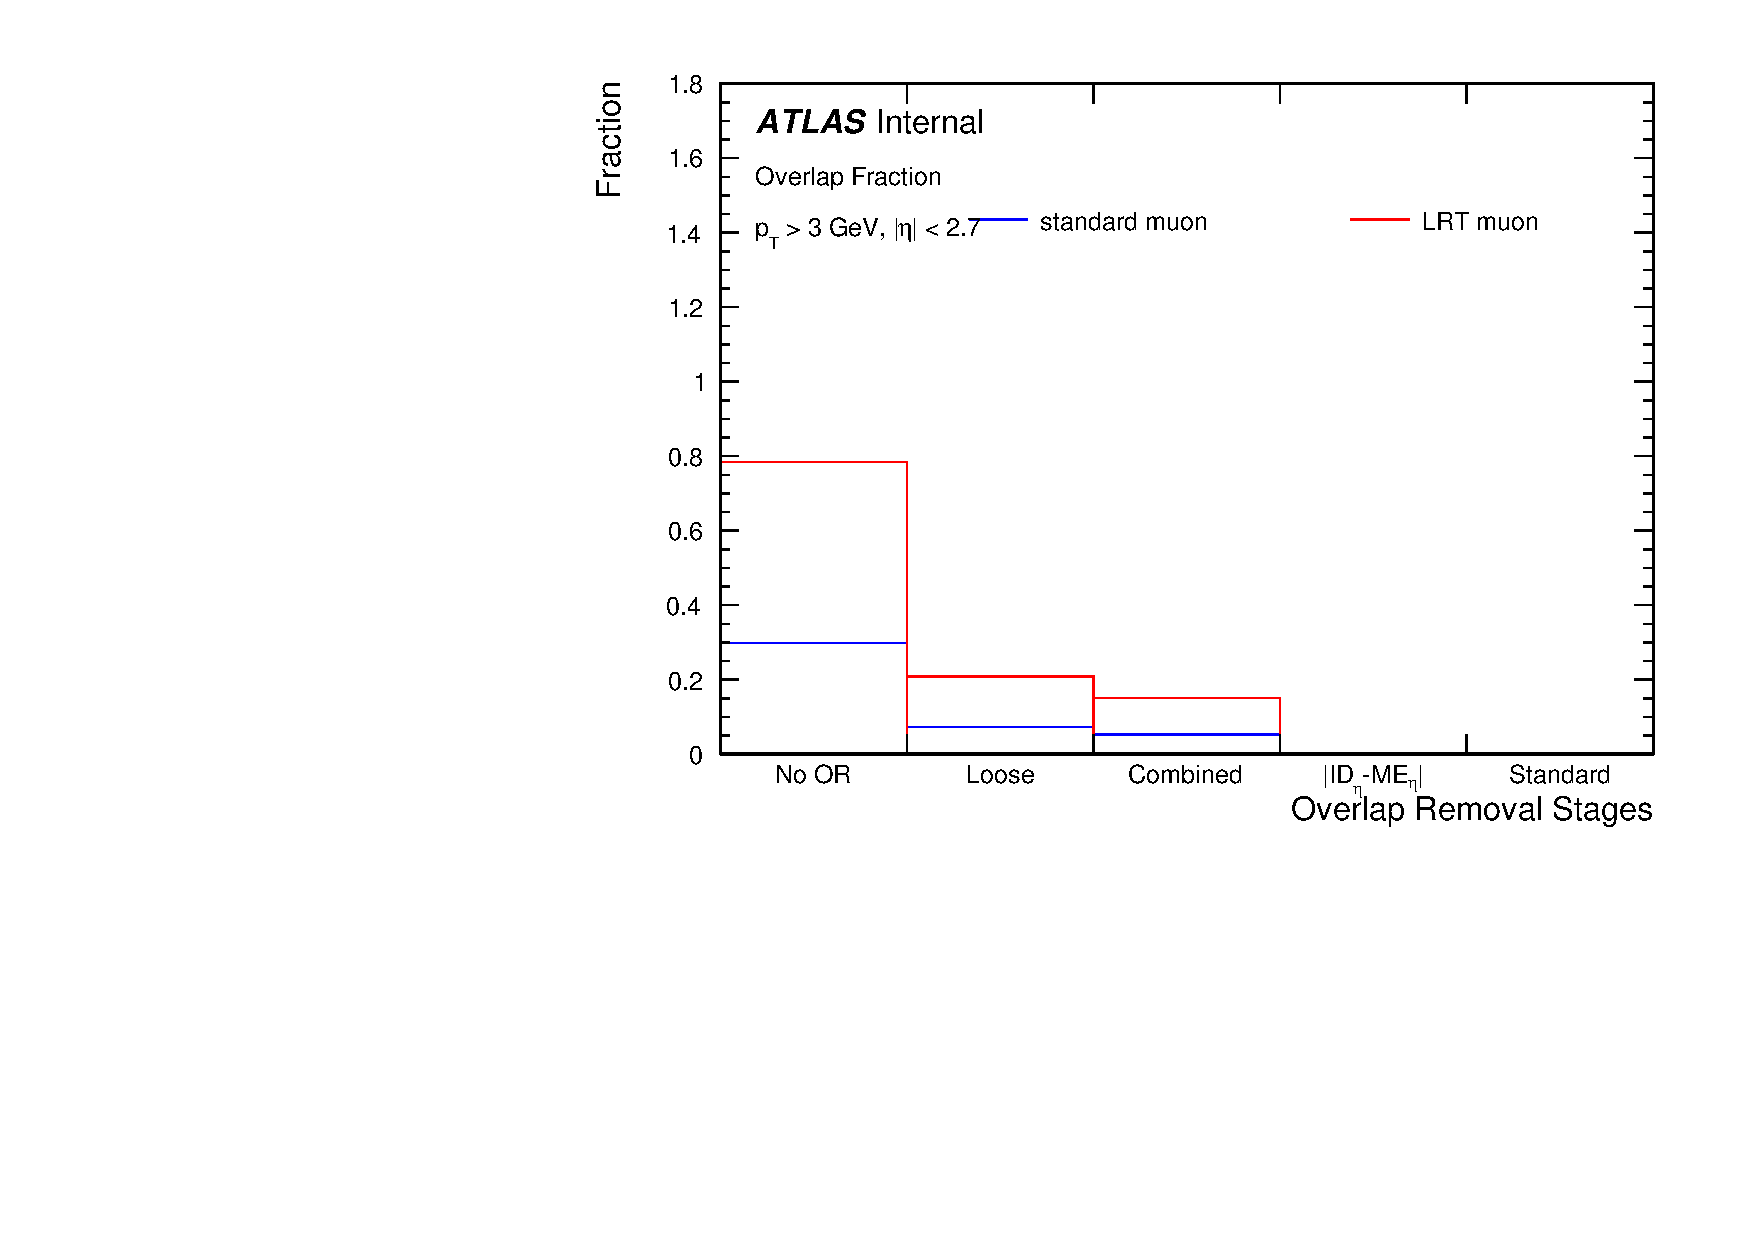
\includegraphics[width=0.8\linewidth]{figures//analysis_overview/plots_muon_overlap_fraction_AllStages.pdf}
    \caption{Fraction of standard and LRT muons that have MS track overlaps at different stages of the overlap removal process.}
    \label{fig:muon_overlap}
\end{figure}

After the standard and LRT muon collections are combined and the overlaps are resolved, they are treated similarly for downstream analysis. Only Combined displaced muons are used in this analysis with the kinematic requirements of \pT$>3$~GeV and $|\eta|<2.5$, both of which are imposed by muon reconstruction and detector constraints. A \texttt{Medium} identification WP is used to identify genuine muons against pion decays. However, the application of the WP is modified for LRT muons. LRT reconstruction has, by design, stringent reconstruction criteria as shown in~\cref{tab:std-lrt-diff}. Hence, the \texttt{Medium} ID WP for LRT muons is slightly modified to not apply the above requirements on the ID tracks while retaining the other cuts.~\Cref{tab:disp_muon_selection} lists the cuts imposed on the identification of displaced muons.

\begin{table}[!ht]
    \centering\small
    \begin{tabular}{cc}
        \hline\hline
        Cut Name & Cut Description \\
        \hline
        Transverse Momentum & \pT $>$ 3 GeV \\
        Pseudo-rapidity & $|\eta|<2.5$ \\
        Muon Type & Combined \\
        Identification Working Point & \texttt{Medium} (w/o ID cuts for LRT muons) \\
        \hline\hline
    \end{tabular}
    \caption{Selection criteria used for displaced muons.}
    \label{tab:disp_muon_selection}
\end{table}


\subsection{Displaced Electrons}
Electrons in the displaced vertex are referred to as displaced electrons. Similar to muons, a combination of standard and LRT electrons are used to identify displaced electrons. The standard and LRT electron reconstruction use the same calorimeter information for each event, and hence, a standard electron and an LRT electron can point to to the same calo-cluster. These \textit{overlaps} are resolved by using the trigger-level identification WPs as defined in~\cite{PERF-2017-01}. Out of an overlapping standard-LRT electron pair, the electron which passes a stricter\footnote{The \texttt{Tight} identification WP has the strictest requirements, followed by \texttt{Medium}, \texttt{Loose}, and \texttt{VeryLoose}.} identification WP requirement is retained. In the case where both the standard and LRT electron pass the same identification WP, the electron reconstructed from the standard pass is kept. The identification WPs used here are further loosened with respect to the trigger-level working points by relaxing the hard requirements on the number of silicon hits in the pixel sub-detectors. 

A \pT threshold of 4.5 GeV is imposed on displaced electrons driven by reconstruction requirements. No cuts beyond those imposed by detector limitations are applied on electron $\eta$. The \texttt{VeryLooseNoPix} identification WP is used for the displaced electrons, which is the same as the \texttt{VeryLooseNoPix} trigger-level identification WP as defined in~\cite{PERF-2017-01} (which already uses a relaxed version of the WPs used for offline electron identification), but with the requirement on the number of silicon pixel hits removed to reduce the bias towards electrons emerging from the IP and add efficiency to electrons from LLP decays. The same identification WP is applied to both standard and LRT electrons. Since the WP imposes very relaxed requirements on the electron, an extra requirement on the compatibility of the \pT of electron object and its corresponding GSF track is imposed to reject mismatches that would rise from photon radiations. Such a cut ensures that the final state identification, which is based on the electron object, and the DV kinematics reconstruction, which is based on the track object, are compatible to each other.~\Cref{tab:disp_electron_selection} lists the cuts imposed on the identification of displaced electrons.

\begin{table}[!ht]
    \centering\small
    \begin{tabular}{cc}
        \hline\hline
        Cut Name & Cut Description \\
        \hline
        Transverse Momentum & \pT $>$ 4.5 GeV \\
        Identification Working Point & \texttt{VeryLooseNoPix}\\
        Momentum Balance & $|\pT^\mathrm{electron}-\pT^\text{GSF track}|/\pT^\mathrm{electron}<0.5$ \\
        \hline\hline
    \end{tabular}
    \caption{Selection criteria used for displaced electrons.}
    \label{tab:disp_electron_selection}
\end{table}

\subsection{b-tagged Jets}
At tree level, the HNL signal process in the fully leptonic final states has no hadronic activity. The leading source of jets in signal events is Initial State Radiation from the incoming partons which then showers to give jets. The chance of hence observing a jet (which have a reconstruction \pT threshold of 20 GeV) is low, and a jet from a b-quark is even lower. This fact is used to define analysis regions rich in correlated background and highly depleted in the signal process.

This analysis uses anti-$k_t$ $\Delta R =0.4$ PFlow jets reconstructed with \pT$>20$~GeV and $|\eta|<4.9$ limited by the calorimeter coverage. Machine learning algorithms are trained to learn about the substructure of jets to classify jets initiated by heavy ($b$ or $c$) quarks against those initiated by light quarks or gluons. In this analysis, the DL1d tagger~\cite{ATL-PHYS-PUB-2022-047} is used to identify the flavor of jets. DL1d is based on a deep neural network. It takes information about the secondary vertex reconstructed inside jets and other low level information about jet substructure and returns a classification score. A cut on the DL1d tagger score of a jet which accepts on average 85\% of jets with b-hadrons, or the 85\% b-jet efficiency WP, is applied to identify jets as either coming from b-quarks, or lighter quark flavors. A jet passing the 85\% WP cut of the DL1d tagger score is called a b-tagged jet or a b-jet.

\subsection{Overlap Removal}
This analysis makes use of reconstructed electron, muon, and jet physics objects. Since the reconstruction chains of these objects runs in parallel, it is possible that such objects share ID tracks or calo-clusters. An overlap removal (where the overlap criteria based on the type of objects in context) step is run after the baseline selection of the physics objects but before using them for analysis. Am overlap removal strategy which favors leptons over jets is used in this analysis. This choice was shown to have a negligible impact on the signal significance in the measured phase space as compared to the standard ATLAS overlap removal strategy. However, a significant increase in the event yield was seen in a non-overlapping analysis region which is used to constrain correlated background contribution. The non-overlapping region is used to collect events with leptons inside jets the statistics of which are increased by using this overlap removal strategy, which led to a better data-driven estimate of the background yield.~\Cref{tab:overlap_removal} lists the rules used for resolving overlaps between physics objects according to the criteria of overlap between them, run sequentially from top to bottom.

\begin{table}[!ht]
    \centering\small
    \begin{tabular}{ccc}
        \hline\hline
        Reject & Against & Overlap Criteria \\
        \hline
        electron$^1$ & electron$^2$ & shared ID track, $\pT^1 < \pT^2$ \\
        muon & electron & is CT-muon and shared ID track \\
        electron & muon & shared ID track \\
        jet & electron & $\Delta R<0.2$ \\
        jet & muon & \#tracks in jet $<$3 and (ghost-associated\footnotemark or $\Delta R<0.2$) \\
        \hline\hline
    \end{tabular}
    \caption{The lepton-favored overlap removal scheme and overlap criteria.}
    \label{tab:overlap_removal}
\end{table}
\footnotetext{Particles are assigned to jets following the ghost-association procedure which consists of assigning them to jets by adding their tracks with infinitesimal \pT to the jet clustering process. A particle is hence ghost-associated to a jet if it is retained after the jet clustering.}

\subsection{Secondary Vertex Reconstruction and Selection}
The track selection, DV reconstruction, and DV selection is facilitated package called Vertex Secondary Inclusive (VSI)~\cite{ATL-PHYS-PUB-2019-013} at the core of which is the vertex reconstruction algorithm, VkalVrt~\cite{Kostyukhin:685551}.

\begin{figure}[!ht]
    \centering
    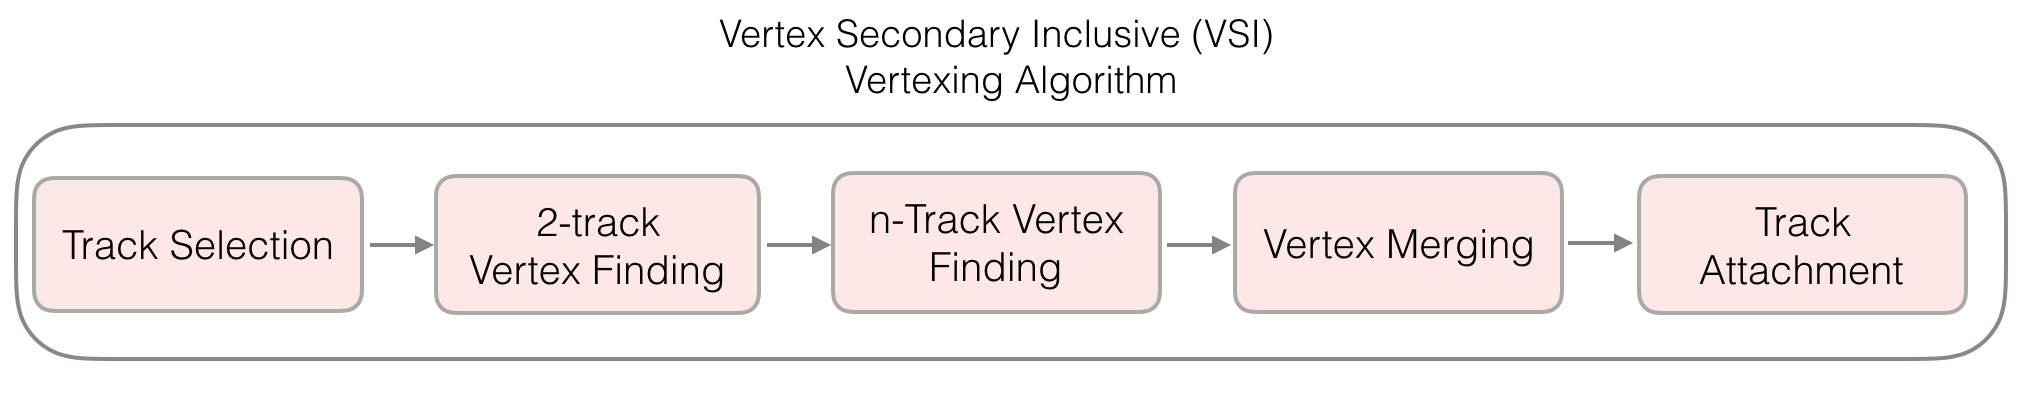
\includegraphics[width=0.8\linewidth]{figures//analysis_overview/vertexing/VSIalg.png}
    \caption{The main steps used for secondary vertex reconstruction in the Vertex Secondary Inclusive algorithm.~\cite{ATL-PHYS-PUB-2019-013}}
    \label{fig:vsi-steps}
\end{figure}

~\Cref{fig:vsi-steps} summarizes the steps followed by VSI for DV reconstruction. This analysis uses the same steps and configurations as outlined in~\cite{ATL-PHYS-PUB-2019-013}, apart from a few but significant notable differences which result in improved signal acceptance and significant reduction in uncorrelated background:
\begin{itemize}
    \item Since the final state probed in this analysis is fully leptonic, the track pool used for seeding is modified to use
    \begin{enumerate}
        \item ID tracks matched to CB or ST muons,
        \item GSF tracks matched to electrons, and
        \item other non-leptonic ID tracks
    \end{enumerate}
    in each event. GSF tracks have better $d_0$ and $z_0$ resolution than standard ID tracks for electrons and hence result in better reconstruction efficiency for DVs with electrons. Other non-leptonic ID tracks are added to all events to expand sensitivity to lepton+track like final states which would result from semi-leptonic decays of the HNL which are planned to be studied in the near future. 
    \item At the two-track vertex finding level, the minimum $|d_0|$ requirement on the pair of tracks is reduced from 2 mm (as is in the standard algorithm) to 1 mm. An error was found in the technical implementation of this cut which led to the accidental acceptance of a significant number of DVs failing this requirement in the 2022 analysis. This error was fixed for this version of the analysis, leading to a significant reduction in correlated background and a near elimination of uncorrelated background.
    \item The track attachment is modified to only consider tracks from the seeding pool. This reduces the unwanted promotion of genuine two-track signal vertices to three-track vertices with one accidental track crossing, say from pileup. Such a change increases signal acceptance since in the downstream analysis, $n$-track vertices are vetoed, where $n>2$.
    \item As a last stage cleaning, all DVs without any tracks matched to leptons are removed.
\end{itemize}

The reconstruction efficiency of DVs is defined as the rate of having a reconstructed vertex matched to an individual HNL decay. To study the tracking and vertexing performance separately from each other, the total efficiency is factorized into independent terms. The efficiencies are defined as follows:
\begin{itemize}
    \item \textbf{Acceptance, $\mathcal{A}$}: fraction of all HNL decays with two charged particles with \pT $>1$~GeV, a true LLP decay $z$ position of $|z|<2720$~mm (inner surface of the last endcap layer), and a transverse distance from the origin of $r_\mathrm{DV}<563$~mm (inner surface of the TRT). The first requirement ensures that the vertex has decay products have large enough momentum to be reconstructed by the tracking algorithm, while the latter two ensure that the HNL was produced within the tracking volume of the ID. The definition of acceptance is purely based on the geometry of the ID without taking into account the limits of track reconstruction, which become more relevant in the next term, the seed efficiency.
    \item \textbf{Seed efficiency, $\varepsilon_\mathrm{seed}$}: fraction of accepted HNL decays having two reconstructed tracks passing the ID track selection requirements. The seed efficiency determines the performance of the object reconstruction algorithms convoluted with the effect of the track seeding cuts.
    \item \textbf{Core efficiency, $\varepsilon_\mathrm{core}$}: fraction of seeded HNL decays having a matched reconstructed vertex.
    The matching of ID tracks to truth particles is based on a weighted scoring of shared detector hits between the track and truth particle trajectories. For each pair of a reconstructed vertex $v$ and a truth HNL decay vertex $l$, a truth-matching score $s$ is computed using the magntitude of the track \pT as a weight. The score is given by:
    \begin{equation}
        s(v, l) \equiv \frac{\sum_{i \in \text { tracks } \in v}\left(\pT^{(i)} \mid \text { descendent of HNL decay } l\right)}{\sum_{i \in \text { tracks } \in v} \pT^{(i)}}
    \end{equation}
    A reconstructed vertex $v$ is said to match to a truth vertex $l$ if the score $s(v,l)>0.5$. The core efficiency represents the true performance of the vertexing algorithm itself with the track acceptance and reconstruction effects factored out.
\end{itemize}

The \textbf{total efficiency ($\varepsilon_\mathrm{total}$)}, is given by
\begin{equation}
    \varepsilon_\mathrm{tot}=\mathcal{A}\cdot\varepsilon_\mathrm{seed}\cdot\varepsilon_\mathrm{core}.
\end{equation}

\begin{figure}[!ht]
    \centering
     \subfloat[Acceptance]{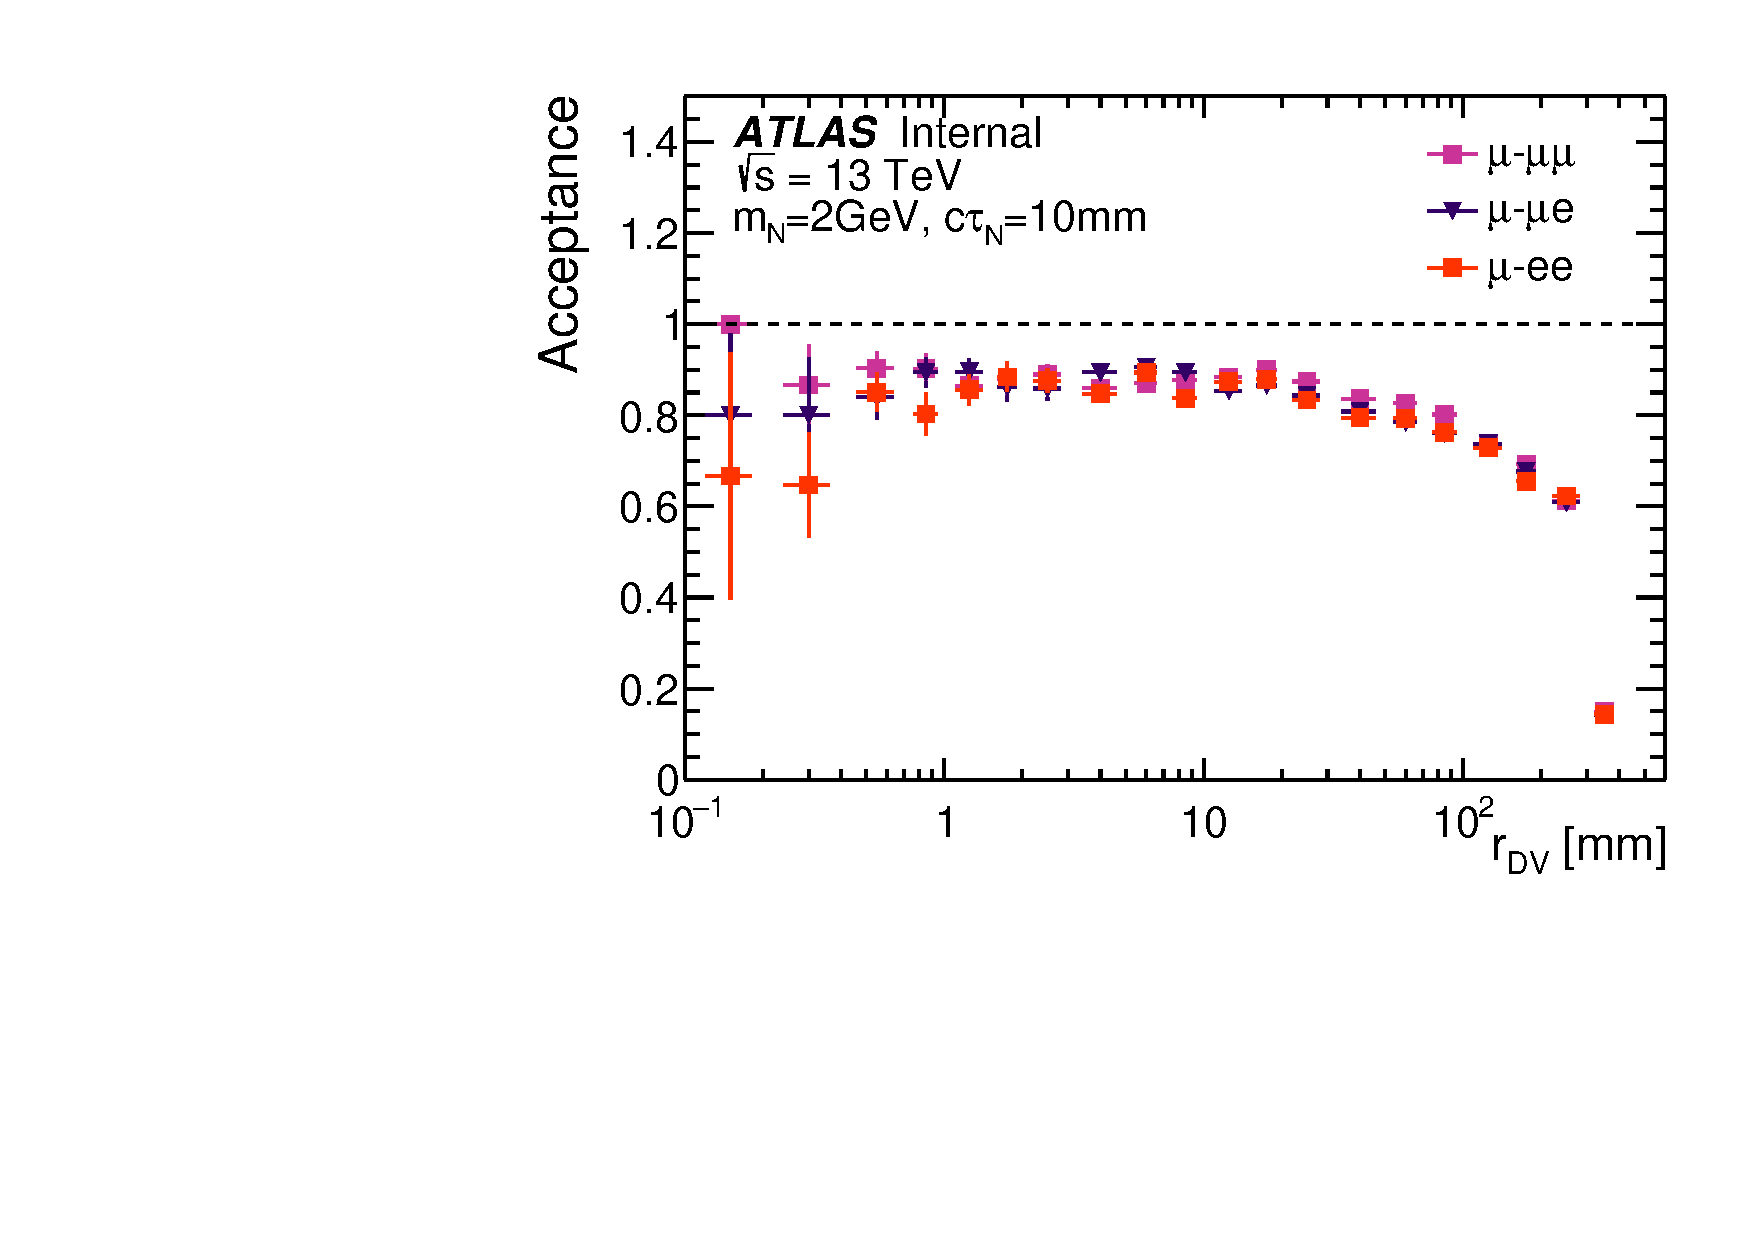
\includegraphics[width=0.45\textwidth]{figures/analysis_overview/vertexing/LC_acc.pdf}}
     \subfloat[Seed efficiency]{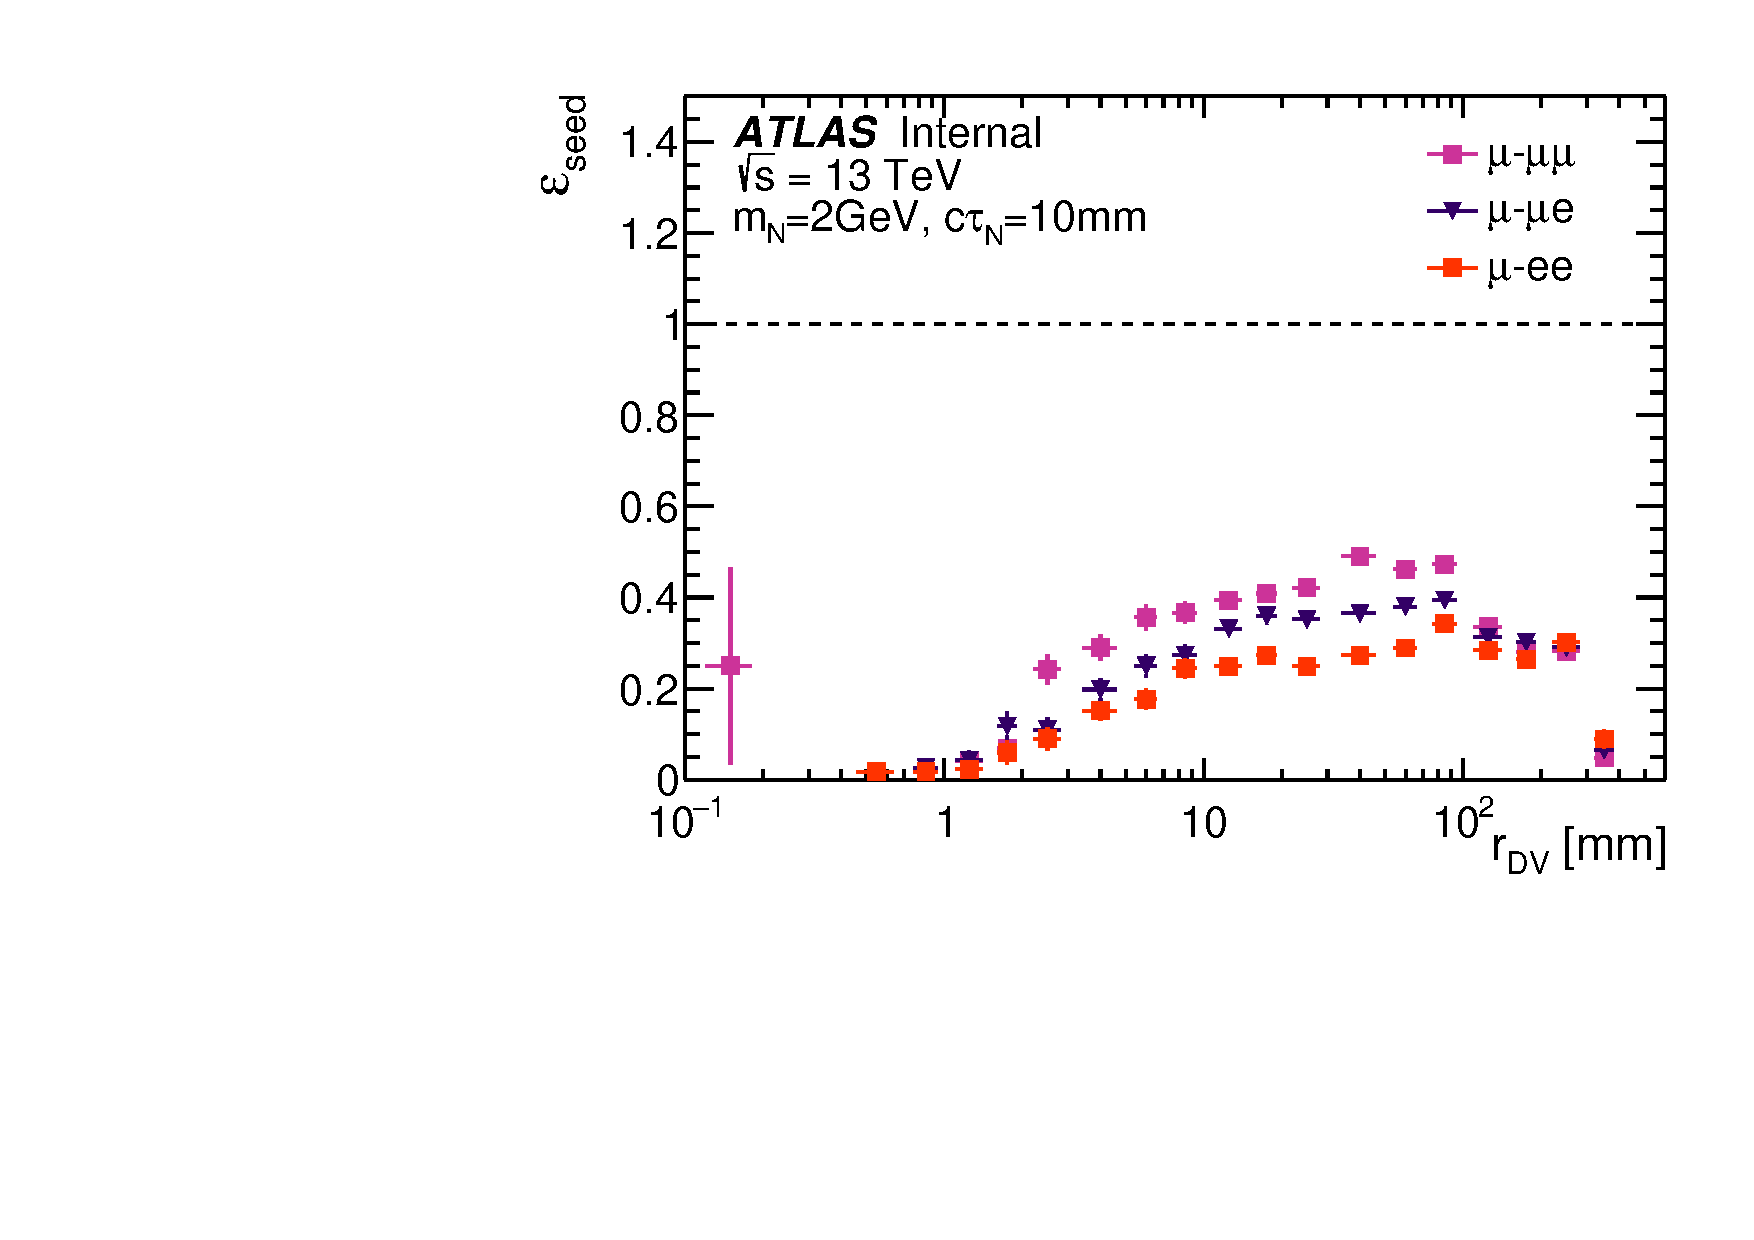
\includegraphics[width=0.45\textwidth]{figures/analysis_overview/vertexing/LC_seed.pdf}} \\
     \subfloat[Core efficiency]{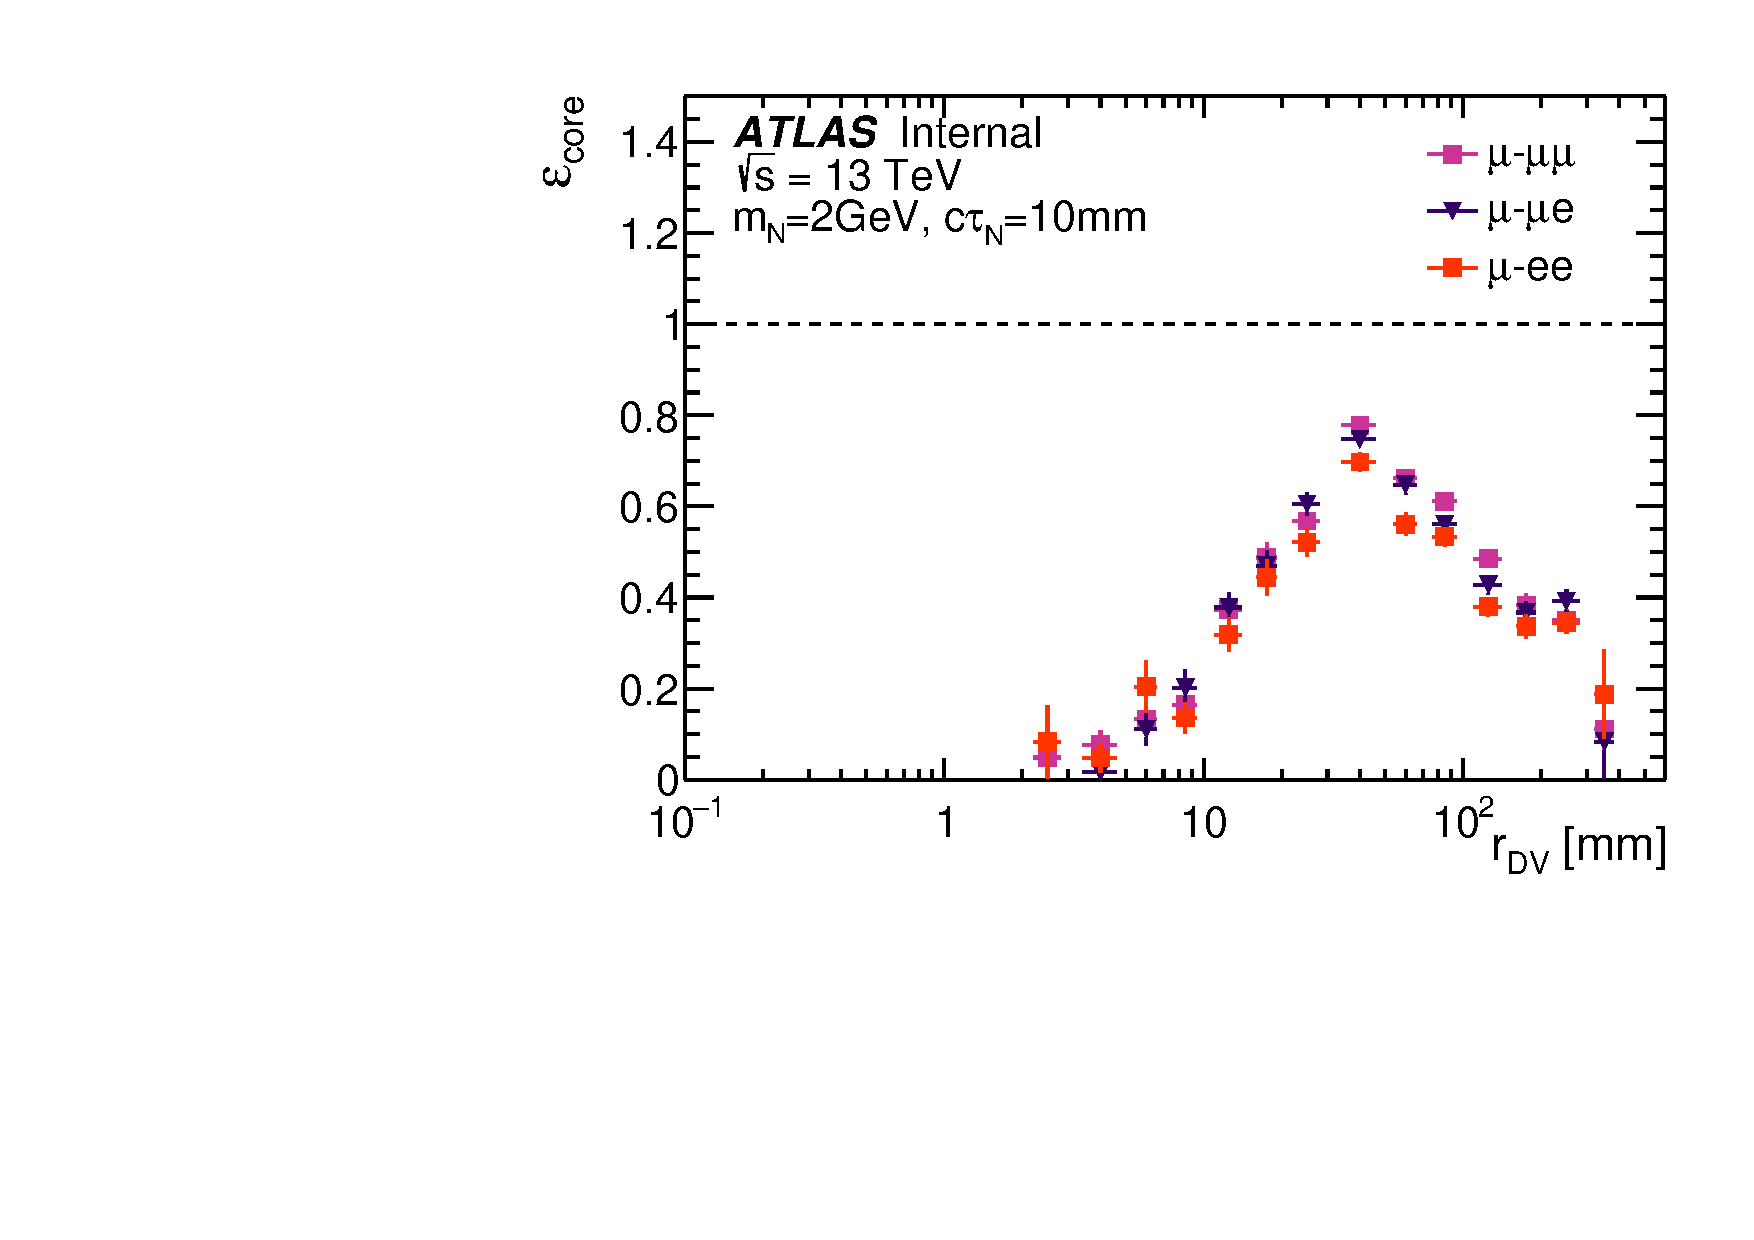
\includegraphics[width=0.45\textwidth]{figures/analysis_overview/vertexing/LC_core.pdf}}
     \subfloat[total efficiency]{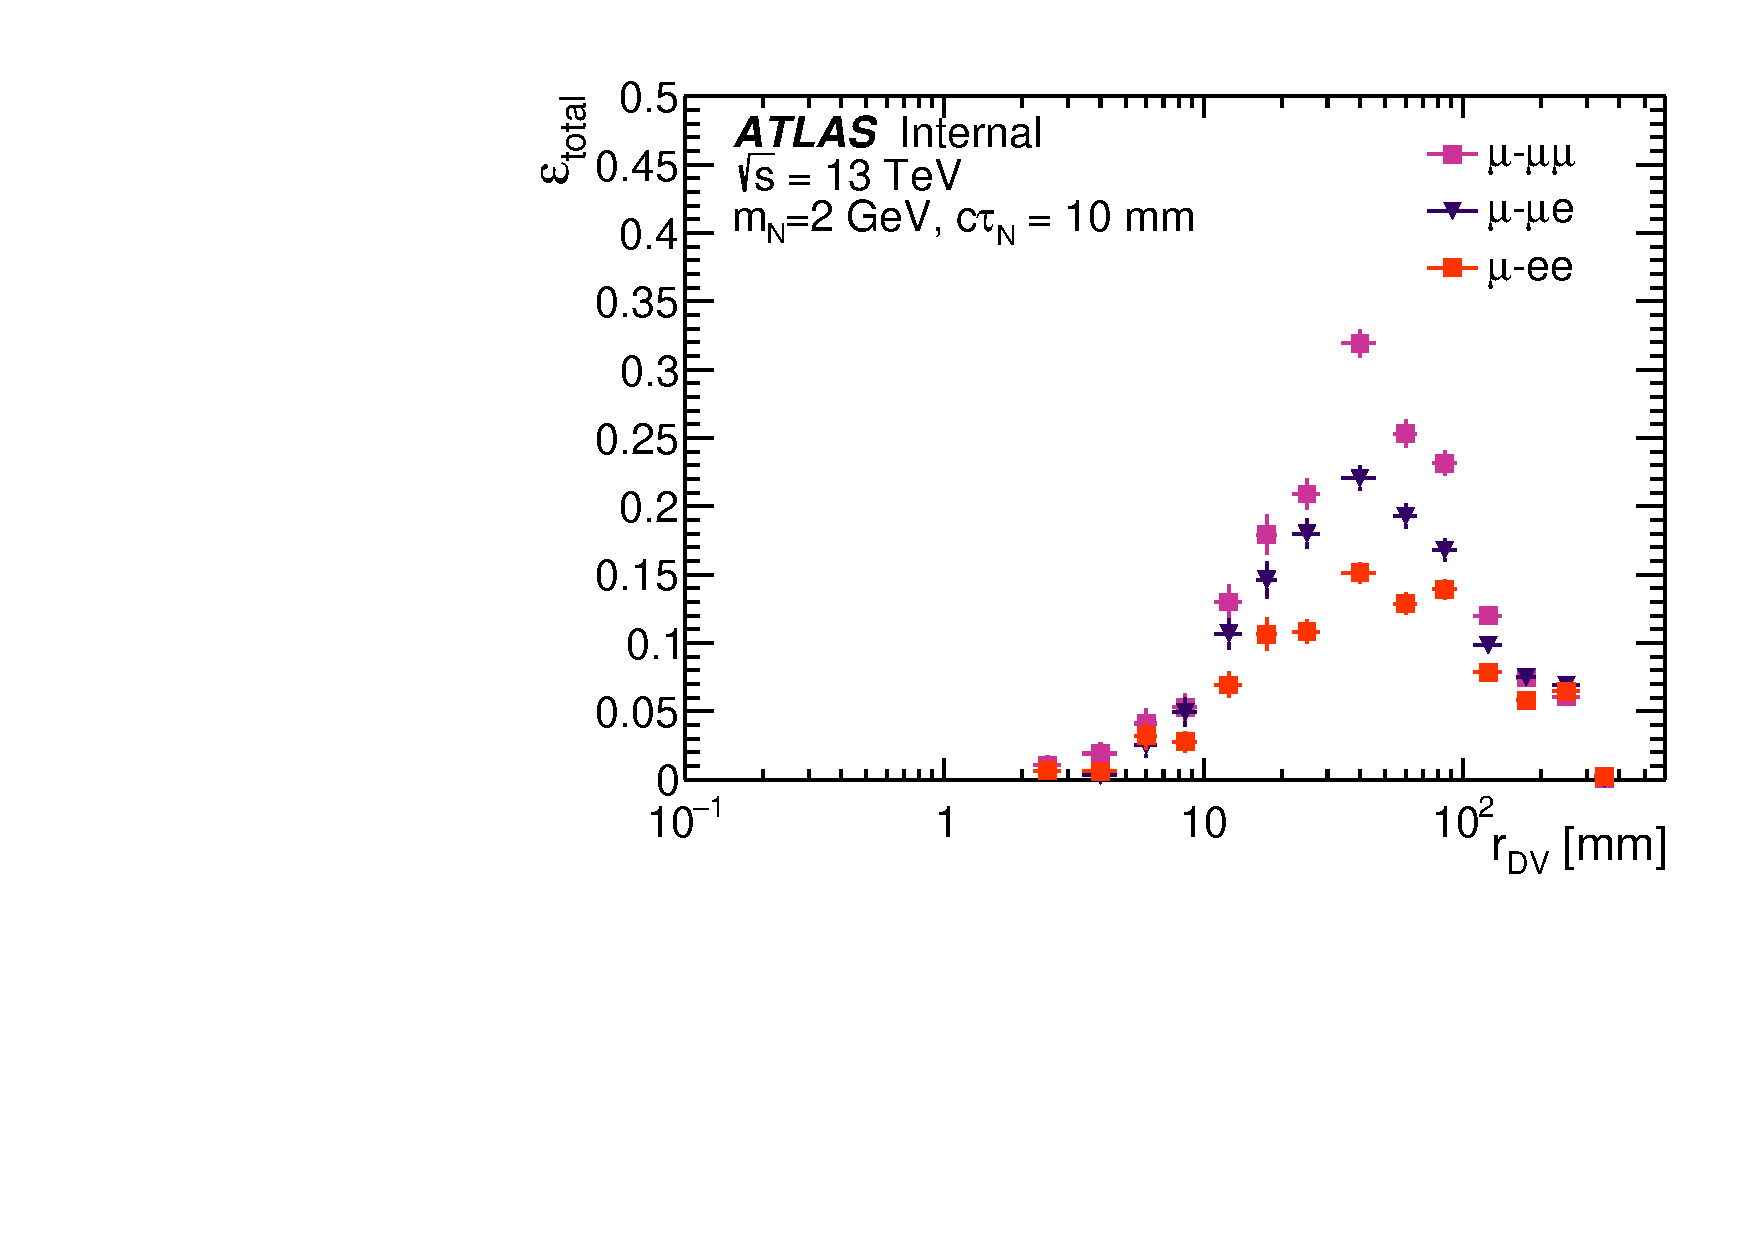
\includegraphics[width=0.45\textwidth]{figures/analysis_overview/vertexing/LC_total.pdf}}
     \caption{The four efficiencies with the custom vertexing configuration as a function of $r_\text{DV}$ evaluated for the \uuu, \uue, and \uee channels with $\mn=2$ GeV, $\ctau=10$ mm.}
     \label{fig:VSILepTrack_sig_eff_LC}
\end{figure}

~\Cref{fig:VSILepTrack_sig_eff_LC} shows the four efficiencies as a function of $r_\text{DV}$, the radial distance of the HNL decay from its origin for a \mn=10 GeV, \ctau=10 mm benchmark HNL signal sample for the three DV flavor combinations $\mu\mu$, $e\mu$, and $ee$ under 2018 pileup and detector conditions. The flavor of the prompt lepton is irrelevant for this study. $\mathcal{A}$ is measured to be uniformly high at $\sim$80\% for all three flavors and falls off at high $r_\text{DV}$ values as the HNL starts to decay outside the ID acceptance. $\varepsilon_\mathrm{seed}$ is highest for $\mu\mu$ followed by $e\mu$ and $ee$. The \pT threshold for electron reconstruction is higher than that for muons (4.5 GeV as compared to 3 GeV), making $\varepsilon_\mathrm{seed}$ lower for LLPs decaying to electrons. Furthermore, a failure in reconstructing any of the two charged particles from the HNL decay would lead to a non-seeded vertex. This, along with the stringent requirements imposed by VSI on track quality, results in relatively low $\varepsilon_\mathrm{seed}$ across DV flavors and the full $r_\text{DV}$ range, with a sharp drop to 0 at $r_\text{DV}>300$~mm due to a drop in track reconstruction efficiency. $\varepsilon_\mathrm{core}$ is similar for all DV flavors. The losses at low $r_\text{DV}$ are driven by the cut on minimum track $|d_0|$. Furthermore, $\varepsilon_\mathrm{core}$ starts dropping at high $r_\text{DV}$ since, for a given mean proper lifetime, the average HNL boost increases with decay radius, resulting in more collimated decay products and a vertex topology which is more challenging to reconstruct. $\varepsilon_\mathrm{total}$ is hence seen to cap at 15-35\% for \mn=10 GeV, \ctau=10 mm HNL decays driven by the DV flavor.

Apart from the effects mentioned above, the DV reconstruction performance also depends on the pileup since a higher incidence of pileup tracks makes it difficult to separate genuine decays from decays from accidental track crossings.~\Cref{fig:vsi-pileup} shows $\varepsilon_\mathrm{total}$ for HNL decays in the \uuu channel for the three different MC campaigns, that correspond to the detector and pileup conditions of different data taking years and have pileup profiles as shown in~\cref{fig:pileup}. The signal DV reconstruction efficiency is observed to be robust against pileup differences whereas the effect is expected to be bigger on background since LRT fake rate increases with pileup.

\begin{figure}[!ht]
    \centering
    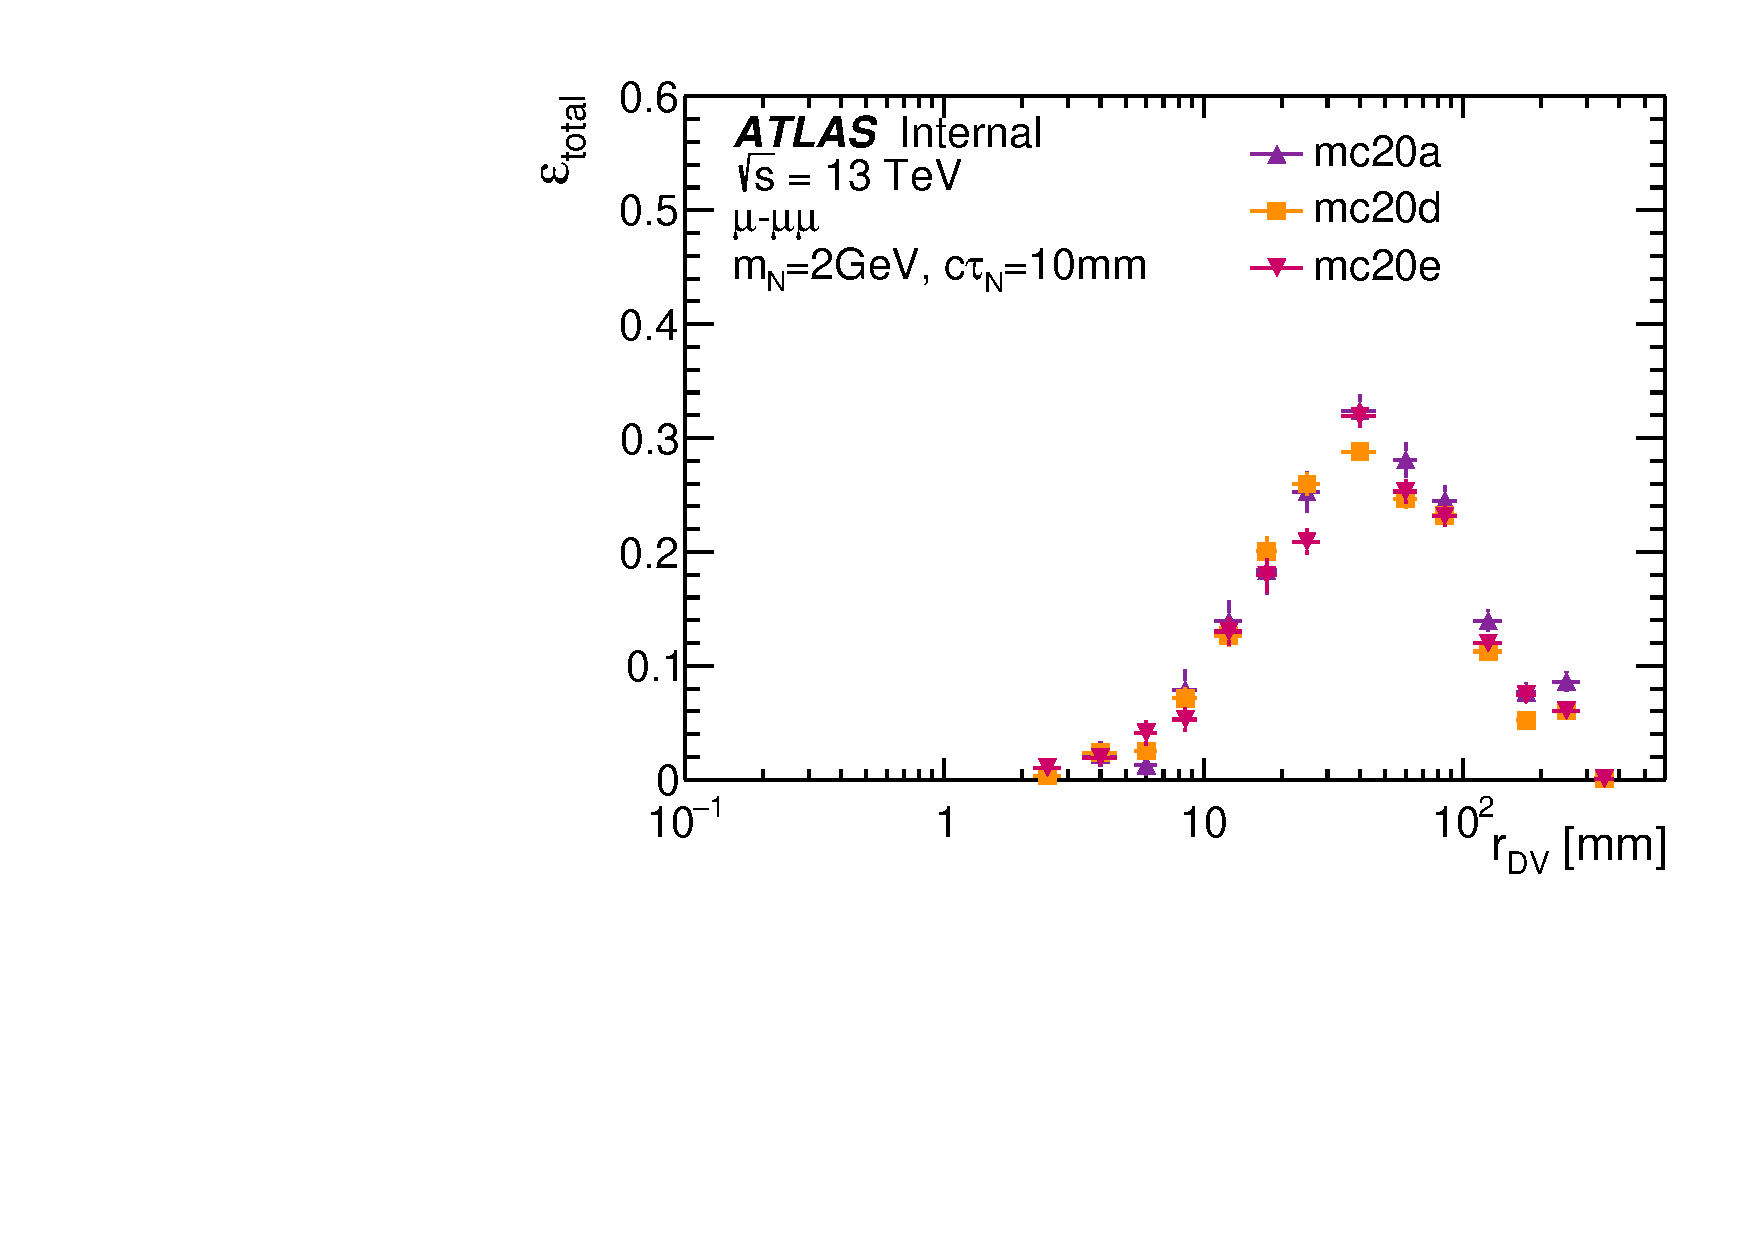
\includegraphics[width=0.5\linewidth]{figures/analysis_overview/vertexing/pileup_eff_total.pdf}
    \caption{Total vertex reconstruction efficiency of $\mn=2$ GeV, $\ctau=10$ mm HNL decays in the \uuu channel for the mc20a, mc20d, and mc20e campaigns.}
    \label{fig:vsi-pileup}
\end{figure}

DVs with exactly two outgoing tracks are considered, where both tracks are required to be either muons or electrons, with the displaced lepton quality requirements imposed on them. The number of events with more than one such DV are found to be negligible, hence the first DV passing these conditions is selected as the HNL candidate. \pT cuts are applied on the DV tracks to reject soft QCD background. Finally, a fiducial selection is applied to the radial position of the DV to ensure the decay happens inside the innermost strip layer of the ID and that the decay has a minimum level of displacement from the PV.~\Cref{tab:dv_selection} summarizes the cuts applied for selection of the DV candidate.

\begin{table}[!ht]
    \centering\small
    \begin{tabular}{ccc}
        \hline\hline
        Cut Name & Cut Description \\
        \hline
        Track multiplicity & exactly 2 \\
        Flavor & $\mu\mu,\,e\mu,\text{or }ee$ \\
        Track \pT & $\pT^\mathrm{lead}>10$~GeV, $\pT^\mathrm{sub-lead}>5$~GeV \\
        %Overlap Removal & $\Delta R(\text{DV tracks}, \text{prompt lep})>0.05$ \\
        Fiducial Cut & 4 mm $<\,r_\mathrm{DV}\,<$~300 mm\\
        \hline\hline
    \end{tabular}
    \caption{Selection criteria used for the displaced vertex.}
    \label{tab:dv_selection}
\end{table}
